\documentclass[a4paper,11pt,twocolumn,twoside]{article}
\usepackage[dvips]{graphicx}
\usepackage{sepln}
\usepackage{changepage}
\usepackage{amsmath}
\usepackage{amssymb}
\usepackage{amsbsy}
\usepackage{svg}
\usepackage{url}
\usepackage{fullname_esp}
\usepackage[utf8]{inputenc}
\usepackage[spanish,es-nosectiondot, es-tabla, es-noindentfirst, es-nolists]{babel}

\input epsf

\setlength\titlebox{4in} %esto por defecto

\title{Extracción automática de estructuras argumentativas en textos de opinión cubanos mediante proyección de etiquetas y aprendizaje profundo}

\author {\textbf{Luis Ernesto Ibarra Vázquez,$^1$} \textbf{Damian Valdés Santiago$^1$}\\
$^1$Facultad de Matemática y Computación, Universidad de La Habana, Cuba\\
% $^2$Universidad de la Habana\\
luise98cu@gmail.com, dvs89cs@matcom.uh.cu\\
}

\seplntranstitle{Automatic extraction of argumentative structures in Cuban opinion texts through label projection and deep learning}

\seplnclave{Extracción de argumentos, procesamiento de lenguaje natural, aprendizaje profundo.} % TODO Seguir en esto

\seplnresumen{
La Extracción de Argumentos se realiza tradicionalmente mediante anotación
manual de expertos en lingüística, lo que demora mucho tiempo. 
Este artículo propone aplicar algoritmos de aprendizaje profundo 
al campo de la Extracción de Argumentos en textos de la prensa cubana, constituyendo el 
primero de su tipo publicado  y adaptado para textos del español de Cuba, hasta donde los autores conocen.
Para ello, 1) se crean conjuntos de datos a partir de provenientes del idioma inglés,
2) se proponen y entrenan los modelos y 3) se anotan
automáticamente las unidades de discurso argumentativas (UDA). Los atributos
utilizados para la representaciones de los textos son aprendidos en el proceso de entrenamiento 
para ajustarse al criterio argumentativo de los datos.
De los conjuntos de datos disponibles, se realizó un análisis de las ventajas y 
deficiencias de cada uno para la anotación de las ``Cartas a la Dirección'' del periódico cubano \textit{Granma}. 
Los resultados obtenidos en la extracción de UDAs alcanzaron valores de
F1 = 0,82 comparados con 0,85 del estado del arte.
En las demás tareas, los resultados no son directamente comparables con los del estado del arte, 
los mejores valores F1 obtenidos fueron 0,56 en la clasificación de UDAs, 0,74 en la predicción
de enlaces y 0,39 en la clasificación de enlaces.
}


\seplnkey{Argument extraction, natural language processing, deep learning.} % TODO Seguir en esto

\seplnabstract{
Argument Extraction is traditionally performed by manual annotation by linguistic experts, which takes lots of time. 
This paper proposes deep learning algorithms to perform the Argument Extraction in 
Cuban press texts, constituting the first of its kind published and adapted for Cuban Spanish texts, as far as the authors 
knowledge. To this end, 1) datasets are created by annotation projection from other ones in English language, 2) models are proposed and trained, 
and 3) automatic annotation of Argumentative Discourse Units (ADUs) is performed. The features used for text representations
are learned in the training process to match the argumentative criteria of the data. From the available data sets, an analysis 
of the advantages and deficiencies of each one was made for the annotation of the ``Letters to the Editor'' of the Cuban newspaper
\textit{Granma}. 
% This analysis was done by the authors and on a subset of 30 of the Letters given the non-existence of an annotated set of it. 
The results obtained in the extraction of ADUs reached values of F1 = 0.82 compared to 0.85 of the state of the art. In 
the other tasks, the results are not directly comparable with those of the state of the art, 
% due to the different approaches taken by the researchers when performing the arguments extraction. 
the best F1 values obtained 
were 0.56 in ADU classification, 0.74 in link prediction and 0.39 in link classification.
}

\firstpageno{1}


\begin{document}

% la siguiente instrucción sólo se debe usar si el abstract sobrescribe el texto
% la longitud variará según se necesite

\setlength\titlebox{22cm} % se aumenta el tamaño del espacio reservado para datos de título


\label{firstpage} \maketitle

%\begin{abstract}
%Resumen del artículo con una sangría a izquierda y derecha de 0.32
%cm, justificado por ambos lados, con tamaño de fuente 11.
%
%\end{abstract}

\section{Introducción}

% Contexto histórico-social donde se desarrolla
% Cuales son las condiciones historicas que hicieron necesarias la creacion de la tesis, o que dieron origen a la problematica de esta

La argumentación es una actividad verbal, social y racional destinada a convencer 
a un crítico razonable de la aceptabilidad de un punto de vista mediante la presentación 
de proposiciones que justifican o refutan la proposición expresada 
en el punto de vista \cite{van2004systematic}. 
% Esta definición concentra en ella 
% partes esenciales de lo que es la argumentación, dicha actividad se encuentra presente
% en varias facetas de la cotidianedad humana, como en la escritura o lectura de documentos y
% en las interacciones sociales de las personas. En resumen, la argumentación está presente 
% cada vez que se plantea un argumento y se trata de que este triunfe en un debate donde 
% se exponen elementos que lo apoyen.



% En la actualidad es necesario tener acceso a la información
% de forma rápida y simple. Esto no siempre es posible dado la gran cantidad de información existente y
% que es generada en cada momento. En caso de tener una vía de acceder a esta, se podrían realizar acciones
% con mayor rapidez y calidad. Con la argumentación, se podría hacer explícitas las razones de las personas 
% al afirmar algo sobre un tema teniendo así su punto de vista individual, y con suficientes personas, colectivo.

% Antecedentes del problema, justificación y motivación. 
% Antecedentes: 
%   Tareas similares que se quedan cortas: Opinion Mining, Citation Mining, Controversy Detection
%   Cómo se ha estudiado primero a mano. Trabajo dificil.
% Justificacion:
%   Limitaciones del trabajo manual
%   Se quiere hacer el trabajo automatico.
%   El proyecto esta integrado en un proyecto nacional  reconocido CORESPUC

Varias tareas en el Procesamiento de Lenguaje Natural (PLN) se han desarrollado alrededor
de diferentes problemas relacionados con 
la argumentación. Entre estas se encuentran: el minado de opiniones, sentimientos y 
emociones expresadas en un texto 
\cite{liu2010sentiment}, la detección de controversias, y la zonificación
argumentativa. 
% Estas tareas muestran cuáles opiniones, puntos de conflictos y roles 
% de argumentos 
% presenta el texto, pero lo realizan de manera separada y no muestran el porqué de estas. 

Es necesario realizar un 
análisis de los argumentos dados, para transformar el texto no estructurado a datos argumentativos 
que permitan el entendimiento de los puntos de vista y de cómo se ``apoyan'' o ``atacan'' entre sí. Este análisis
es posible realizarlo manualmente o utilizando programas
especializados para la anotación, aunque la práctica ha demostrado que este proceso requiere 
de una gran cantidad de tiempo y de personal calificado \cite{eger2018cross}. 
% Con la inmensa cantidad de datos 
% que se genera a diario este análisis es impracticable de realizar de forma manual, por esto se 
% estudian y crean métodos para automatizar esta tarea.

% Breve presentación de la problemática. 
%   Por todo lo anterior nace la EA, rama de PLN ..., definir tareas de la EA, tocar los enfoques realizados
% (No es el estado del arte aunque se puede hablar un poco de él) Elementos involucrados en el punto de vista cientifico, lleva corpus.

La Extracción de Argumentos (EA) es la rama del PLN encargada
del estudio de métodos para la extracción automática de las estructuras argumentativas de 
los textos y su posterior procesamiento \cite{lawrence2020argument}. Esta tarea se divide en 
cuatro subtareas fundamentales: i) la extracción y ii) clasificación de las componentes 
argumentativas del texto, y iii) la extracción y 
iv) clasificación de las relaciones entre estas. 

% Esta es un área de investigación muy activa donde estas tareas han sido abordadas de diferentes maneras:
% desde modelos secuenciales \cite{palau2009argumentation,goudas2015argument} hasta 
% \textit{end-to-end} \cite{eger2017neural}, desde el uso de clasificadores clásicos 
% como \textit{Naive Bayes} o máquinas de soporte vectorial (SVM, en inglés) \cite{niculae2017argument}, \cite{stab2017parsing} hasta el uso de 
% aprendizaje profundo \cite{galassi2021deep}, \cite{mayer2020transformer}.

La EA se caracteriza por la poca disponibilidad de datos anotados y 
por la heterogeneidad de las 
anotaciones. Además, la gran mayoría de los estudios realizados en el campo se encuentran en 
idiomas como el inglés, alemán o chino \cite{eger2018cross}. 
En español, se reportan pocas investigaciones del análisis de los argumentos \cite{esteve2020mineria} y, en 
Cuba, no se encontró ninguna referencia, según la búsqueda de literatura científica
realizada por los autores.

% Actualidad, novedad e importancia teórica y práctica. 
%   En español no tiene mucho estudio. Citar casos del español, para Cuba ninguno
%   Creación de un corpus anotado el cual se podrá mejorar con el tiempo

% Diseño teórico.
%    Problema: 
%    Objeto de Investigación: Procesamiento de Lenguaje Natural
%    Campo de acción: Linguistica computacional
%    Hipótesis o preguntas científicas
%    Objetivos generales y específicos
%       General: Diseño e implementación de un algoritmo para el estudio de la argumentación en el periódico digital \textit{Granma}
%       Especifico Construcción del corpus de los periódicos: Crawler, Anotación (scpaCy).
%       Especifico Implementacion de la interfaz gráfica para consultar los resultados.

El objetivo, de esta investigación es proponer un algoritmo basado en aprendizaje profundo 
para la extracción y análisis de estructuras argumentativas en textos 
de la prensa cubana (en particular, la sección ``Cartas a la Dirección'' del períodico \textit{Granma}), 
constituyendo el primero de su tipo publicado y adaptado para
textos del español de Cuba, hasta donde los autores conocen. 
Para lograr dicho objetivo, en primer lugar, es necesario obtener mediante \textit{crawling} los textos a analizar del sitio 
web del periódico \textit{Granma}. Luego, se proponen algoritmos de aprendizaje automático capaces de realizar las tareas 
de EA sobre estos textos, que requiren conjuntos 
de datos anotados en español sobre los cuales se puedan entrenar.

Para la extracción
de argumentos se presentan dos modelos, el primero se encarga de la segmentación y clasificación
de las componentes argumentativas mediante la clasificación de los \textit{tokens} en etiquetas BIOES, que % TODO citar las etiquetas BIOES
delimitan y clasifican las unidades de discurso argumentativas (UDA). En el segundo, se analizan 
las posibles relaciones entre UDAs de manera independiente para saber si están relacionadas o no y
el tipo de relación existente. Los modelos utilizan 
redes neuronales convolucionales (CNN, en inglés), \textit{Long Short Term Memory} (LSTM, en inglés) \cite{hochreiter1997long} y \textit{Conditional Random Field} (CRF, en inglés) \cite{lafferty2001conditional}
como elementos principales en sus arquitecturas, además se emplean vectores GloVe \cite{pennington2014glove} para la representación
de las palabras. 
% Los algoritmos propuestos se aplican a textos del periódico \textit{Granma}, 
% en específico, se enfoca en su sección de ``Cartas a la Dirección''.

% Este es un modelo secuencia a secuencia en el cual las palabras 
% son vectorizadas por sus características morfológicas mediante el uso de redes neuronales convolucionales
% (CNN) y \textit{Long Short Term Memory} (LSTM), por su información
% semántica mediante \textit{embeddings} \textit{Global Vectors} (GloVe) y por su información 
% estructural mediante su parte de la oración, estas 
% secuencias son procesadas por una red LSTM bidireccional y sus atributos son usados por una capa 
% de \textit{Conditional Random Field} (CRF)
% para su clasificación final en etiquetas BIOES, con información adicional para la clasificación de las 
% unidades de discurso argumentativas (UDA). El segundo modelo está encargado de la extracción y clasificación 
% de las relaciones entre las UDAs. En él se utilizan las representaciones GloVe de las palabras en las secuencias 
% y su distancia argumentativa para la clasificación de una tupla en la que su primer elemento 
% constituye el texto candidato de donde parte la relación o fuente y el segundo, el texto candidato a recibir la 
% relación u objetivo, en el tipo de relación existente entre estos elementos. La entrada es procesada mediante 
% una LSTM bidireccional y módulos de atención cruzada entre los elementos de la fuente y los elementos del objetivo.
% Para la visualización se crea un ambiente de desarrollo con la herramienta Brat\footnote{\url{https://brat.nlplab.org/}},
% la cual permite realizar las tareas requeridas a los datos anotados por los modelos.

% En resumen, se presenta un estudio de la argumentación en español al realizar la extracción de 
% argumentos en prensa, tributando además conjuntos de datos anotados en español que puede servir
% para un estudio más profundo sobre los esquemas argumentativos presentes en estos textos.

% Estructura del trabajo % TODO para el final

El artículo se divide en varias secciones. Primero, se presentan las definiciones 
relativas a la argumentación y la EA. Luego, se presenta 
un estado del arte de la EA con una discusión de las
ventajas y desventajas de cada enfoque y se introduce la proyección de corpus. Más adelante, 
se presentan los modelos propuestos para resolver el problema en 
cuestión. A continuación se muestran los resultados del entrenamiento de los modelos y en 
la anotación de los textos de ``Cartas a la Dirección''. Finalmente, se exponen las conclusiones y 
recomendaciones de la investigación.

% ARGUMENTACION

% \section{Argumentación}

% Para el estudio de la argumentación han surgido algunos enfoques que componen un marco teórico 
% en donde se sustentan las investigaciones. Las ideas de \cite{perelman1969rhetoric} están
% enfocadas en un análisis de la retórica en donde se estipula que la teoría de la argumentación
% responde a provocar o aumentar la adhesión de las personas a las tesis presentadas, por medio de 
% técnicas discursivas. En \cite{toulmin_2003} se considera como argumento todo aquello que ofrece, 
% o todo lo que es utilizado, para justificar o refutar una proposición. En este último, se toma 
% una perspectiva más racional y deductiva de la argumentación, dando como resultado lo que se 
% conoce como el Método de Toulmin.

% La argumentación es un tema tratado desde la antigüedad, Aristóteles lo defendía como la 
% habilidad de, dada una pregunta, considerar los elementos útiles para persuadir a alguien, algo
% similar a la retórica. De una perspectiva más contemporánea surgen las ideas de 
% \cite{perelman1969rhetoric}
% enfocadas en un análisis de la retórica en donde se estipula que la teoría de la argumentación
% responde a provocar o aumentar la adhesión de las personas a las tesis presentadas, por medio de 
% técnicas discursivas. En 
% \cite{toulmin_2003}
% se considera como argumento todo aquello que ofrece, 
% o todo lo que es utilizado, para justificar o refutar una proposición. En este último, se toma 
% una perspectiva más racional y deductiva de la argumentación, dando como resultado lo que se 
% conoce como el Método de Toulmin. 

% \subsection{Método de Toulmin}

% Este método divide los argumentos en seis partes: afirmación 
% (\textit{claim}), fundamento (\textit{grounds}), justificación (\textit{warrant}), calificador 
% (\textit{qualifier}), refutación (\textit{rebuttal}) y respaldo (\textit{backing}).
% Mediante las afirmaciones se conoce el argumento principal que el autor quiere probar a la audiencia,
% estas son respaldadas con fundamentos, siendo estos las evidencias y hechos en que se apoya el autor.
% Las justificaciones pueden estar explícitas o implícitas y son suposiciones que vinculan los
% fundamentos con las afirmaciones, estas a su vez pueden ser respaldadas por conocimiento.
% El esquema introduce la posibilidad de otra situación válida a la establecida en las afirmaciones
% mediante la refutación. Los calificadores son usados para dar más información de la calidad o seguridad
% de las afirmaciones dadas. 
% Un ejemplo\footnote{Extraído de
% 	\cite{toulminArgument}.
% } de este esquema es:

% \begin{adjustwidth}{25pt}{25pt}
% 	[\textit{Se escucharon ladridos y aullidos en la distancia}]$_{\mathrm{fundamento}}$, 
% 	[\textit{probablemente}]$_{\mathrm{calificador}}$
% 	[\textit{haya perros en las cercanías}]$_{\mathrm{\text{afirmación}}}$.
% \end{adjustwidth}

% En este ejemplo, además de las partes explícitas, se encuentran partes implícitas como la justificación 
% (\textit{los perros son animales que ladran y aúllan}), el respaldo (\textit{se sabe que existen perros en la zona}) y 
% la refutación (\textit{puede ser que hayan lobos o coyotes cerca}).

% Este método crea una definición compacta que ayuda a los investigadores a enfocar su búsqueda 
% en las diferentes categorías definidas. Además, engloba de manera comprensible un tema tan complejo 
% como la argumentación al tomar en cuenta gran parte de los elementos presentes en el razonamiento
% realizado para llegar a conclusiones, incorporando incluso elementos probabilísticos en el proceso. 

% \subsection{Rasgos lingüísticos}

% Los rasgos lingüísticos son aquellas características que se encuentran presentes en los textos 
% que hacen que estos se clasifiquen argumentativos \cite{venegas2005hacia}. Con 
% la identificación de estos se hace la tarea de extracción más sencilla y con un marco teórico 
% que respalde las decisiones tomadas. Ejemplos de rasgos presentes en textos argumentativos:

% \begin{enumerate}
% 	\item Marcas de orden que introducen párrafos: \textit{primero}, \textit{segundo}, \textit{por un lado},
% 	      \textit{por otra parte}, \textit{finalmente}.
% 	\item Comillas y citas: citar palabras que refuercen la intervención recurriendo a autoridades
% 	      o personajes.
% 	\item Nexos que expresan causa o consecuencias: \textit{ya que}, \textit{porque}, \textit{pues},
% 	      \textit{con motivo de}, \textit{gracias a}, \textit{considerando que}, \textit{por lo tanto}, \textit{de manera que}.
% \end{enumerate}

% Estos rasgos además de dar indicación de la existencia de argumentos dan pie para conocer las relaciones
% entre estos y los tipos de argumentos. Por ejemplo, \textit{por lo tanto}, implica que lo que viene 
% a continuación es una conclusión apoyada en lo dicho anteriormente en el texto. Algo parecido
% sucede con \textit{ya que}, en este caso implica que lo siguiente es un argumento que se encuentra 
% relacionado con lo mencionado antes.

% En
% \cite{venegas2005hacia}
% se determinan 16 categorías y 51 rasgos lingüísticos, dando una idea 
% de la gran variedad de marcadores presentes en la argumentación.

\section{Extracción de Argumentos} %% RESUMED

La EA consiste en la identificación y extracción 
automática de las estructuras de inferencia y 
razonamiento expresadas como argumentos presentes en el lenguaje natural \cite{lawrence2020argument}.
La EA permite dar respuesta a este problema presentando
los argumentos y cómo sus relaciones justifican las posiciones del hablante. Dicho problema está constituido por diferentes 
estructuras y se compone de distintas tareas necesarias para su solución.

Existen diferentes estudios que conforman una metodología de análisis para
identificar los argumentos. El modelo de Toulmin \cite{toulmin_2003} introduce categorías 
con distintas funciones dentro de la argumentación. En 
el idioma español existen rasgos lingüísticos que, además de dar indicación de la existencia de argumentos, 
dan pie para conocer las relaciones entre estos y los tipos de argumentos. \namecite{venegas2005hacia}
determina 16 categorías y 51 rasgos lingüísticos, dando una idea de la gran variedad de marcadores 
presentes en la argumentación.

\subsection{Estructuras Argumentativas}

Las estructuras argumentativas son las partes de la argumentación de los textos y sus relaciones.
Estas se componen de dos elementos principales: las Unidades de Discurso Argumentativas (UDAs) y los enlaces
o relaciones existentes entre estas. Las UDAs corresponden a la unidad mínima de argumentación, definida 
como un segmento de texto que juega un solo rol para el argumento analizado, y es 
delimitado por segmentos vecinos que tienen roles diferentes o ningún rol \cite{stede2018argumentation}.

Las UDAs se relacionan entre sí conformando el proceso de inferencia y razonamiento del argumento.
Tanto los enlaces como las UDAs son clasificados en dependencia de su rol en la argumentación. Estas clasificaciones 
parten de los conceptos de afirmación, declaración controversial y parte central del argumento, y premisa, % TODO Poner referencias a los conceptos, o eliminarlos
razones que la justifican o refutan, y en las relaciones de ataque y apoyo. 

\subsection{Tareas de extracción de argumentos}

Dada la definición de estructuras argumentativas y que el objetivo de la EA es extraerlas,
se conciben las siguientes tareas principales:

\begin{enumerate}
	\item Extracción de UDAs: separar los segmentos de texto que formarán parte de la UDA.
	\item Clasificación de UDAs: asignar una categoría argumentativa a la UDA segmentada.
	\item Extracción de relaciones entre las UDAs: determinar si están relacionadas las UDAs o no.
	\item Clasificación de relaciones entre las UDAs: asignar una categoría a la relación extraída.
\end{enumerate}

% A continuación se presenta un ejemplo en donde se encuentran realizadas dichas tareas, clasificando
% las UDAs en afirmación y premisa y la relación en apoyo:

% \begin{adjustwidth}{25pt}{25pt}
% 	En primer lugar, [\textit{el correo electrónico puede contar como uno de los resultados
% 	más beneficiosos de la tecnología moderna}]$_{\mathrm{\text{Afirmación}}}$. [\textit{Años atrás, las personas pagaban gran cantidad de dinero para
% 	enviar sus cartas y sus pagos estaban sujetos al peso de sus cartas o paquetes y muchos accidentes podrían 
% 	causar problemas que causarían que el correo no fuera enviado}]$_{\mathrm{Premisa, -1, apoyo}}$.
% \end{adjustwidth}

% El -1 representa la distancia argumentativa, que es la cantidad de UDAs del texto que separan la 
% UDA fuente del objetivo \cite{galassi2021deep}, en caso de ser negativa (positiva) el objetivo se encuentra 
% antes (después) que la fuente.

% Puede observarse que las estructuras argumentativas de un texto constituyen un grafo dirigido 
% en donde sus nodos representan las UDAs y están etiquetados con su tipología, y sus aristas representan las 
% relaciones entre las UDAs. Dichas aristas se anotan con el tipo de relación existente entre ambas 
% (Figura \ref{fig:arg_struct}).

% \begin{figure}[h]
% 	\centering
% 	\includesvg[width=7cm]{Graphics/Estructuras_argumentativas.svg}
% 	\caption{Estructuras Argumentativas.}
% 	\label{fig:arg_struct}
% \end{figure}

% INVESTIGACIONES PREVIAS

\subsection{Variantes para la Extracción de Argumentos}

Varias investigaciones han dado respuesta a los problemas asociados a EA, mostrando
una variedad en enfoques y métodos. Para la segmentación de las UDAs se ha separado
en oraciones y luego clasificado cada una en si es UDA o no mediante algoritmos como 
\textit{Naive Bayes} (NB) y máquinas de soporte vectorial (SVM, en inglés) \cite{palau2009argumentation,goudas2015argument}.
Otras aproximaciones para esta tarea consiste en la clasificación en etiquetas BIO
de los \textit{tokens} del texto \cite{goudas2015argument,stab2017parsing,eger2017neural} y en el uso de
reglas basadas en anotaciones lingüísticas \cite{dykes2020reconstructing}.

En las tareas de predicción y clasificación de enlaces se han empleado gramáticas libre de contexto 
basadas en anotaciones de los \textit{tokens} \cite{palau2009argumentation}. SVM y aprendizaje profundo han sido utilizados para clasificar 
las posibles relaciones dos a dos \cite{goudas2015argument,galassi2021deep}, en \namecite{goudas2015argument}
se optimiza la estructura final con un problema de optimización lineal en enteros.

Las UDAs y las relaciones han sido representadas de diferentes maneras, ya sea por 
atributos escogidos a mano mediante conocimiento experto \cite{palau2009argumentation,goudas2015argument}, como
por atributos aprendidos por los algoritmos en la fase de entrenamiento \cite{eger2017neural,galassi2021deep}.

% \subsection{Variantes para la Extracción de Argumentos}

% Varias investigaciones han dado respuesta a los problemas asociados a EA, mostrando
% una variedad en enfoques y métodos.\\

% En \cite{palau2009argumentation} se analizan las UDAs a nivel de oraciones.
% Este propone \textit{Naive Bayes} (NB) y máquinas de soporte vectorial (SVM, en inglés) para la clasificación
% de oraciones de oraciones en argumentativas o no. Las oraciones son representadas
% on un vector conformado de atributos a partir de conocimiento experto de la argumentación. En
% la predicción de relaciones utilizan una gramática libre de contexto.

% % \begin{itemize}
% % 	\item Se analizan las UDAs a nivel de oraciones.
% % 	\item Propone \textit{Naive Bayes} (NB) y \textit{Support Vector Machine} (SVM) para la clasificación
% % 	de oraciones de oraciones en argumentativas o no.
% % 	\item Las oraciones se representan con un vector conformado de atributos a partir de conocimiento experto
% % 	de la argumentación.
% % 	\item Para la predicción de relaciones utilizan una gramática libre de contexto. 
% % \end{itemize}

% % En \cite{palau2009argumentation} se propone
% % el uso de modelos como \textit{Naive Bayes} (NB) y \textit{Support Vector Machine} (SVM)
% % para la clasificación de 
% % oraciones en argumentativas o no y en su rol argumentativo en caso de que sea argumentativa. En este
% % se asume que las componentes argumentativas son oraciones completas. Para la predicción de relaciones
% % se usa un enfoque basado en reglas con la creación de una Gramática Libre de Contexto. Las representaciones
% % de las oraciones consisten en atributos creados a mano, dado el conocimiento experto sobre la argumentación
% % en el tema tratado, elementos como adverbios, verbos, signos de puntuación, palabras clave, estadísticas del texto
% % (tamaño de oración, distancia media de palabras) son usados para la extracción y clasificación de las UDAs, además,
% % se usan también como base en la creación de las reglas de la gramática para la extracción de relaciones.

% En \cite{goudas2015argument} las UDAs son analizadas a nivel de oración.
% Se propone usar NB, \textit{random forest}, regresión logística y SVM 
% para la clasificación en argumentativas o no. De las oraciones argumentativas,
% se extraen las secciones con carga argumentativa mediante anotación de etiquetas 
% BIO con un campo condicional aleatorio (CRF, en inglés). Se predicen las relaciones como un 
% problema de clasificación de pares de UDAs en donde emplean SVM. También
% utilizan atributos escogidos a mano mediante conocimiento experto para la representación de 
% las oraciones y palabras.

% % \begin{itemize}
% % 	\item Se analizan las UDAs a nivel de oraciones.
% % 	\item Propone usar NB, \textit{random forest}, regresión logística y SVM 
% % 	para la clasificación en argumentativas o no.
% % 	\item En las oraciones argumentativas, se extraen las secciones con carga argumentativa 
% % 	mediante anotación de etiquetas BIO con un campo condicional aleatorio (CRF, en inglés).
% % 	\item Se predicen las relaciones como un problema de clasificación de pares de UDAs en donde emplean
% % 	SVM. 
% % 	\item Utilizan atributos escogidos a mano mediante conocimiento experto para la representación de 
% % 	las oraciones y palabras.
% % \end{itemize}

% % \cite{goudas2015argument} al igual que \cite{palau2009argumentation} clasifica a las oraciones como
% % argumentativas o no, mediante diferentes clasificadores como NB, \textit{Random Forest}, Regresión
% % Logística y SVM. Sin embargo, \cite{goudas2015argument} aumenta la grandularidad de la segmentación al permitir
% % la extracción de los segmentos que contienen la carga argumentativa de dentro de las oraciones previamente clasificadas
% % como tal, esto se realiza mediante la extracción de etiquetas BIO de las oraciones con el uso de un 
% % CRF. La predicción de las relaciones es modelado como un problema de clasificación
% % usando SVM para clasificar pares de UDAs en relacionados o no. Atributos creados a mano 
% % son usados en la extracción de UDAs; entre estos están posición de la oración en el texto, cantidad de verbos, comas, adverbios,
% % palabras, entidades en la oración, también se emplean listas que guardan entidades relacionadas con el dominio 
% % específico y palabras clave indicadoras de frases argumentativas. 

% En \cite{stab2017parsing} las UDAs son extraídas mediante un modelo CRF con clasificación en etiquetas BIO.
% La predicción y clasificación de relaciones se modela conjuntamente mediante dos SVMs,
% optimizando la estructura final con un problema de optimización lineal en enteros. Los \textit{tokens}
% y las UDAs están representados por vectores con atributos seleccionados por expertos.

% % \begin{itemize}
% % 	\item Se extraen las UDAs mediante un modelo CRF con clasificación en etiquetas BIO.
% % 	\item La predicción y clasificación de relaciones se modela conjuntamente mediante dos SVMs,
% % 	optimizando la estructura final con un problema de Optimización Lineal Entero.
% % 	\item Las representaciones vectoriales de los \textit{tokens} y las UDAs se constituyen por atributos 
% % 	seleccionados a mano por conocimiento experto.
% % \end{itemize}

% % \cite{stab2017parsing} proponen un mecanismo de segmentación basado en CRF. La clasificación
% % y predicción de relaciones se modela conjuntamente con dos clasificadores SVM y un problema
% % de Optimización Lineal Entero que encuentra la mejor estructura y asegura una disposición arbórea. En la segmentación
% % de las UDAs, se extraen por cada \textit{token} su posición en el texto, si precede o sucede a un signo de puntuación, su parte de
% % la oración, la probabilidad de que sea el comienzo de una UDA dado sus \textit{tokens} anteriores, entre otros. Para la extracción
% % y clasificación de relaciones se proponen otros conjuntos de atributos como la cantidad de sustantivos comunes entre
% % las componentes fuente y el objetivo, la presencia de indicadores argumentativos, representaciones vectoriales de \textit{tokens} 
% % entre otros.

% En \cite{eger2017neural} se presentan enfoques \textit{end-to-end}, modelando el problema como
% uno de anotación secuencia a secuencia (capa de clasificación CRF al final), también
% como uno de análisis sintáctico de dependencia (\textit{dependency parsing}) \cite{kiperwasser2016simple}
% y además mediante el reconocimiento de entidades nombradas, en donde las entidades son las UDAs.
% Las representaciones de los \textit{tokens} son aprendidas por el algoritmo mediante la 
% aplicación de capas de CNN sobre los caracteres.

% % \begin{itemize}
% % 	\item Presenta un enfoques \textit{end-to-end}, modelando el problema como:
% % 	\begin{itemize}
% % 		\item Anotación secuencia a secuencia (capa de clasificación CRF al final).
% % 		\item Análisis sintáctico de dependencia (\textit{dependency parsing}) \cite{kiperwasser2016simple}.
% % 		\item Reconocimiento de entidades nombradas, en donde las entidades son las UDAs.
% % 	\end{itemize}
% % 	\item Las representaciones de los \textit{tokens} son aprendidas por el algoritmo mediante la 
% % 	aplicación de capas de CNN sobre los caracteres.
% % \end{itemize}

% % En \cite{eger2017neural} trabajan el problema de EA como uno \textit{end-to-end}. 
% % Para esto presentaron varias propuestas, entre ellas se encontraba
% % modelar el problema como uno de secuencia a secuencia, usando RNN como 
% % LSTM en versiones bidireccionales capturando información desde ambos lados de la secuencia.
% % Para la representación de las palabras se extrajo información morfológica de las palabras mediante 
% % la aplicación de una CNN a los caracteres de estas,
% % al final, realizan la clasificación de la secuencia con un CRF. 
% % Realizaron experimentos al modelar el problema como uno de \textit{Dependency Parsing} \cite{kiperwasser2016simple}. Este problema
% % consiste en construir un árbol de dependencia que codifique las estructuras argumentativas. En este 
% % se tiene que decidir entre varias opciones (\textit{shift}, \textit{reduce}) en dependencia del contenido de la pila y del \textit{buffer}
% % para la confección del árbol.
% % El problema fue modelado también como un problema de reconocimiento de entidades nombradas, en donde las entidades son las UDAs.

% En \cite{dykes2020reconstructing} proponen métodos sobre reglas basadas en anotaciones lingüísticas (partes de la oración, lemas de palabras, etc.) 
% para la extracción de argumentos. Dada las reglas creadas y el tipo
% de datos con que se trabaja (cadenas de texto pequeñas); estos algoritmos tienden a tener una alta precisión aunque 
% bajo recobrado, esto no es un gran problema en conjuntos de datos grandes, pero en conjuntos de menor tamaño o estructura 
% más compleja pierden efectividad.

% % \begin{itemize}
% % 	\item Se proponen métodos sobre reglas basadas en anotaciones lingüísticas (partes de la oración, lemas de palabras, etc.) 
% % 	para la extracción de argumentos. 
% % \end{itemize}

% % En \cite{dykes2020reconstructing} se proponen métodos basados en reglas para la extracción de argumentos sobre
% % textos en Twitter. Estos métodos se centran en la confección de reglas basadas en anotaciones lingüísticas como
% % partes de la oración y lemas de palabras. La recuperación está basada en los esquemas argumentativos comunes presentes
% % en los textos. Dada las reglas creadas y el tipo
% % de datos con que se trabaja, o sea, cadenas de texto pequeñas; estos algoritmos tienden a tener una alta precisión aunque 
% % bajo recobrado, esto no es un gran problema en conjuntos de datos grandes, pero en conjuntos de menor tamaño o estructura 
% % más compleja pierden efectividad.

% En \cite{galassi2021deep} se propone el uso de redes residuales y mecanismos de atención
% para la clasificación de UDAs y la predicción y clasificación de los enlaces. En este
% se clasifica conjuntamente el tipo de UDA y la relación entre estas. Los textos son 
% representados como una secuencia de vectores GloVe para los \textit{tokens}, por lo que 
% no interviene conocimiento experto en la representación.

% \begin{itemize}
% 	\item Propone el uso de redes residuales y mecanismos de atención.
% 	\item Clasifica conjuntamente el tipo de UDA y la relación entre estas.
% 	\item Representa el texto como una secuencia de vectores GloVe para los \textit{tokens}.
% \end{itemize}

% \cite{galassi2021deep} propone el uso de redes residuales y mecanismos de atención
% para la creación de un modelo que, conjuntamente, clasifica el tipo de UDA y la relación existente entre estas.
% Este trabajo define el concepto de distancia argumentativa, añadiéndolo como característica y asume que las UDAs ya fueron 
% extraídas. En este caso, además de la distancia argumentativa, las secuencias son representadas 
% vectorialmente con GloVe.

% Cada enfoque tiene su ventaja y desvantaja, el modelado secuencial de los problemas, introduce
% una propagación de error en las etapas posteriores e impide que el modelo obtenga toda la información de
% la fuente original. Para la obtención de reglas y atributos creados por expertos 
% se necesita una cantidad 
% de tiempo y recursos, y puede ser más difícil de escalar y mantener que representaciones aprendidas
% automáticamente en el proceso de entrenamiento, estas se pueden moldear a los distintos
% tipos de situaciones y esquemas presentes en los datos.

En los modelos propuestos (ver secciones \ref{ssec:segm_clsf_uda} y \ref{ssec:pred_clsf_enlaces}), gran parte de las representaciones son aprendidas en el proceso de 
entrenamiento y las que se agregan de forma manual casi no influyen en la escalabilidad del sistema.
Cuando se trata de unir los resultados de los dos modelos, hay una propagación de errores, 
aunque se utiliza el modelado de problemas conjuntos para minimizarlo.
% Dado que se tienen dos modelos independientes se tiene una propagación del error al unir los resultados 
% del primero con el segundo, aunque se hace uso del modelado conjunto de problemas para evitar esta 
% situación en las tareas de extracción y clasificación de UDAs y extracción y clasificación de relaciones.

% En resumen, se contemplan disímiles enfoques al problema de EA desde una perspectiva enmarcada en modelos 
% simbólicos, estadísticos y neuronales en versiones tanto secuenciales como \textit{end-to-end}. 
% Cada uno de estos modelos presentan sus ventajas y desventajas a la hora de construirlos, 
% extenderlos y comprender su funcionamiento. En modelos simbólicos se presenta una alta
% precisión en dominios específicos debido a que se construyen teniendo en cuenta reglas específicas a un
% contexto dado. Estos modelos son poco escalables y difíciles de mantener ya que sus reglas son construídas
% a mano y dicho proceso requiere de conocimiento experto y tiempo. Los modelos estadísticos 
% se caracterizan por usar conjuntos de atributos creados a mano, dichos atributos son difíciles
% de encontrar, calcular y pueden no poseer relevancia en otros contextos diferentes a los que fueron creados,
% además, la necesidad de conocimiento experto es necesaria para su confección. Los modelos neuronales poseen
% una mayor adaptabilidad, en estos la entrada puede ser codificada en una representación que es aprendida por
% el mismo algoritmo, permitiendo su uso en esquemas argumentativos con características diferentes. Los modelos simbólicos y 
% estadísticos poseen la ventaja de poder explicar el porqué de los resultados devueltos cosa que se vuelve casi
% imposible en modelos neuronales.

% Dado que la EA es un proceso en el cual se necesita pasar por varias tareas, estas deben de ser completadas
% de alguna forma. Una manera de completarlas es hacerla una a la vez, independiente una de otra y pasándole
% la salida de etapas anteriores a las etapas siguientes. Esta manera secuencial de realizar las 
% tareas es bastante simple y ayuda a la creación de modelos simples y con tareas bien definidas, aunque trae consigo 
% la propagación de los errores a través del proceso y el no aprovechamiento de las interrelaciones entre variables 
% computadas de procesos anteriores. También requiere de la construcción, entrenamiento y evaluación de varios modelos.
% En cambio un enfoque \textit{end-to-end} poseen la habilidad de modelar el problema 
% desde su inicio hasta su final de manera conjunta, mediante \textit{Multi-Task Learning} (MTL) se modelan
% las tareas de manera conjunta creando un solo modelo complejo con una propagación de error menor.

\subsection{Proyección de etiquetas} %% RESUMED

% La EA no presenta una gran cantidad de datos anotados en español con los cuales se pueda realizar 
% un entrenamiento, además de esto la gran mayoría de corpus existentes se encuentran en lenguajes como inglés o alemán.
% Para desarrollar la EA en otros lenguajes, como el español, se han investigado diferentes variantes
% para la construcción de conjuntos de datos, a partir de los conjuntos de datos ya existentes.

La proyección de etiquetas es un algoritmo donde se 
transfieren las etiquetas de un corpus anotado a nivel de \textit{tokens} en un lenguaje origen hacia su traducción en un
lenguaje objetivo. En \cite{eger2018cross} se propone un algoritmo de proyección a partir de las alineaciones de 
palabras. El proceso se divide en varias partes:

\begin{enumerate}
	\item Traducción automática de oraciones: proceso de
	traducir automáticamente texto de un lenguaje fuente a un lenguaje objetivo.
	\item Alineación de palabras: consiste en asignar las palabras del lenguaje fuente
	a sus equivalentes generadas en el lenguaje objetivo.
	\item Proyección de etiquetas: consiste en transformar las etiquetas de las palabras en la secuencia origen
	hacia las palabras de la secuencia destino tomando como datos las alineaciones entre estas.
\end{enumerate}

% A continuación se presentan un ejemplo\footnote{Extraído del corpus de \cite{stab2017parsing}.} del 
% procedimiento descrito. En estos se observa el proceso de alineación
% de los índices de los \textit{tokens} en inglés con sus respectivos \textit{tokens} en español, esta relación puede ser de 
% muchos a muchos y no necesariamente se conserva el orden de las palabras. Luego se observa el paso de 
% etiquetas del lenguaje fuente al objetivo basadas en la información de la alineación. 

% \begin{adjustwidth}{25pt}{25pt}
% 	Firstly$_0$ ,$_1$ people$_2$ normally$_3$ have$_4$ lots$_5$ of$_6$ things$_7$ to$_8$ do$_9$ .$_{10}$ \\\\
% 	En primer$_0$ lugar$_0$ ,$_1$ la gente$_2$ normalmente$_3$ tiene$_4$ muchas$_5$ cosas$_7$ que$_8$ hacer$_9$ .$_{10}$
% \end{adjustwidth}
% \text{}\newline
% \begin{adjustwidth}{25pt}{25pt}
% 	Firstly$_O$ ,$_O$ people$_B$ normally$_I$ have$_I$ lots$_I$ of$_I$ things$_I$ to$_I$ do$_I$ .$_O$ \\\\
% 	En$_O$ primer$_O$ lugar$_O$ ,$_O$ la$_O$ gente$_B$ normalmente$_I$ tiene$_I$ muchas$_I$ cosas$_I$ que$_I$ hacer$_I$ .$_O$
% \end{adjustwidth}


% \subsection{Traducción de oraciones}

% La Traducción Automática consiste en el proceso de usar inteligencia artificial para
% traducir texto de un lenguaje fuente a un lenguaje objetivo sin la intervención humana.
% En la actualidad, este campo ha dado un gran paso pasando de modelos estadísticos a modelos
% neuronales obteniendo traducciones de una alta calidad sin variar significativamente de la humana, 
% condición necesaria para una buena proyección \cite{eger2018cross}.

% Este primer paso de la proyección de corpus consiste en traducir todas las oraciones existentes 
% en el conjunto de datos hacia el lenguaje objetivo. 
% A continuación se muestra una oración en inglés y su traducción al español\footnote{Extraído del corpus de \cite{stab2017parsing}.}:

% \begin{adjustwidth}{25pt}{25pt}
% 	Firstly , people normally have lots of things to do . \\
% 	En primer lugar , la gente normalmente tiene muchas cosas que hacer .
% \end{adjustwidth}

% \subsection{Alineación de palabras}

% La alineación de palabras consiste en encontrar las palabras generadas en el lenguaje objetivo por las 
% palabras en el lenguaje fuente.
% Algoritmos basado en modelos bayesianos, como FastAlign \cite{dyer2013fastalign}, 
% y Cadenas de Markov-Monte Carlo, como EFEMARAL \cite{ostling2016efficient} se ubican entre
% las primeras herramientas para la solución del problema. 
% Modelos más recientes se han enfocado en explotar las representaciones
% vectoriales de palabras y el uso de métodos de atención para la extracción de las
% alineaciones \cite{dou2021word}. Algunas consideraciones sobre el proceso: las relaciones 
% formadas entre palabras pueden ser de tipo muchos a muchos, además de no tener el mismo orden de la 
% oración inicial o incluso no estar relacionadas directamente con una palabra en la oración objetivo.
% Estas consideraciones dan una medida de la dificultad de la tarea en cuestión.
% En el ejemplo siguiente se observa el resultado de las herramientas de alineación, en este 
% las palabras en el idioma de origen (inglés) están anotadas con su posición en la oración y 
% las palabras en el idioma objetivo (español) están anotadas con la posición de la palabra que 
% la originó en el idioma origen:

% \begin{adjustwidth}{25pt}{25pt}
% 	Firstly$_0$ ,$_1$ people$_2$ normally$_3$ have$_4$ lots$_5$ of$_6$ things$_7$ to$_8$ do$_9$ .$_{10}$ \\
% 	En primer$_0$ lugar$_0$ ,$_1$ la gente$_2$ normalmente$_3$ tiene$_4$ muchas$_5$ cosas$_7$ que$_8$ hacer$_9$ .$_{10}$
% \end{adjustwidth}
% \begin{adjustwidth}{25pt}{25pt}
% 	Firstly$_O$ ,$_O$ people$_B$ normally$_I$ have$_I$ lots$_I$ of$_I$ things$_I$ to$_I$ do$_I$ .$_O$ \\
% 	En$_O$ primer$_O$ lugar$_O$ ,$_O$ la$_O$ gente$_B$ normalmente$_I$ tiene$_I$ muchas$_I$ cosas$_I$ que$_I$ hacer$_I$ .$_O$
% \end{adjustwidth}


% \subsection{Proyección de etiquetas}

% La proyección de etiquetas consiste en transportar las etiquetas de las palabras en la secuencia origen
% hacia las palabras de la secuencia destino tomando como datos las alineaciones entre estas. En \cite{yarowsky2001inducing}
% se trata el problema de proyección de frases nominales, estas frases tienen como característica que son resistentes
% a ser divididas en caso de ser traducidas, y aunque evidencian 
% cambios en el orden de las palabras, mantienen la misma ventana; dicha propiedad se cumple para las UDAs también.
% La proyección de UDAs es más simple en dado
% que solamente se tiene en cuenta la ventana y las etiquetas en estas son constantes, no pasa con la proyección en
% frases nominales, las cuales pueden cambiar dentro de una ventana, por lo que algoritmos más simples existen
% para esta tarea \cite{eger2018cross}. En el ejemplo de proyección están anotadas las etiquetas originales en formato BIO
% de las palabras de la oración en el lenguaje origen (inglés) y se muestra el
% resultado de proyectar estas al lenguaje objetivo utilizando los resultados de la alineación de palabras:

% \begin{adjustwidth}{25pt}{25pt}
% 	Firstly$_O$ ,$_O$ people$_B$ normally$_I$ have$_I$ lots$_I$ of$_I$ things$_I$ to$_I$ do$_I$ .$_O$ \\
% 	En$_O$ primer$_O$ lugar$_O$ ,$_O$ la$_O$ gente$_B$ normalmente$_I$ tiene$_I$ muchas$_I$ cosas$_I$ que$_I$ hacer$_I$ .$_O$
% \end{adjustwidth}

\section{Segmentación y clasificación de UDAs}

Las tareas de segmentación y clasificación de UDAs se resuelven conjuntamente. Para esto se modela 
como un problema secuencia a secuencia cuyo objetivo es asignar, a los \textit{tokens} extraídos del documento 
entrada, una etiqueta BIOES para segmentar las UDAs. Para la clasificación del tipo 
de UDA, al conjunto de etiquetas BIES se le añade otra etiqueta que representa el tipo de UDA. Con 
este esquema se obtiene una cantidad de etiquetas $|\{B,I,E,S\}| \cdot |Clasificaciones \, de \, UDA| + |\{O\}|$.

% Esta primera parte se modela como un problema secuencia a secuencia cuyo objetivo es asignar a los \textit{tokens} 
% extraídos del documento entrada una etiqueta BIOES para segmentar las UDAs. Para la clasificación del tipo 
% de UDA, al conjunto de etiquetas BIES se le añadieron las clasificaciones que presenta el corpus entrenante.
% En el siguiente ejemplo se muestra una salida del modelo presentando las clasificaciones de
% $A$ como argumento y $P$ como premisa:

% \begin{adjustwidth}{25pt}{25pt}
% 	En$_O$ primer$_O$ lugar$_O$ ,$_O$
% 	[\textit{el$_{B-A}$}
% 	\textit{correo$_{I-A}$}
% 	\textit{electrónico$_{I-A}$}
% 	\textit{puede$_{I-A}$}
% 	\textit{contar$_{I-A}$}
% 	\textit{como$_{I-A}$}
% 	\textit{uno$_{I-A}$}
% 	\textit{de$_{I-A}$}
% 	\textit{los$_{I-A}$}
% 	\textit{resultados$_{I-A}$}
% 	\textit{más$_{I-A}$}
% 	\textit{beneficiosos$_{I-A}$}
% 	\textit{de$_{I-A}$}
% 	\textit{la$_{I-A}$}
% 	\textit{tecnología$_{I-A}$}
% 	\textit{moderna$_{E-A}$}]
% 	.$_{O}$
% 	[\textit{Años$_{B-P}$}
% 	\textit{atrás$_{I-P}$}
% 	\textit{,$_{I-P}$}
% 	\textit{las$_{I-P}$}
% 	\textit{personas$_{I-P}$}
% 	\textit{pagaban$_{I-P}$}
% 	\textit{gran$_{I-P}$}
% 	\textit{cantidad$_{I-P}$}
% 	\textit{de$_{I-P}$}
% 	\textit{dinero$_{I-P}$}
% 	\textit{para$_{I-P}$}
% 	\textit{enviar$_{I-P}$}
% 	\textit{sus$_{I-P}$}
% 	\textit{cartas$_{I-P}$}
% 	\textit{y$_{I-P}$}
% 	\textit{sus$_{I-P}$}
% 	\textit{pagos$_{I-P}$}
% 	\textit{estaban$_{I-P}$}
% 	\textit{sujetos$_{I-P}$}
% 	\textit{al$_{I-P}$}
% 	\textit{peso$_{I-P}$}
% 	\textit{de$_{I-P}$}
% 	\textit{sus$_{I-P}$}
% 	\textit{cartas$_{I-P}$}
% 	\textit{o$_{I-P}$}
% 	\textit{paquetes$_{I-P}$}
% 	\textit{y$_{I-P}$}
% 	\textit{muchos$_{I-P}$}
% 	\textit{accidentes$_{I-P}$}
% 	\textit{podrían$_{I-P}$}
% 	\textit{causar$_{I-P}$}
% 	\textit{problemas$_{I-P}$}
% 	\textit{que$_{I-P}$}
% 	\textit{causarían$_{I-P}$}
% 	\textit{que$_{I-P}$}
% 	\textit{el$_{I-P}$}
% 	\textit{correo$_{I-P}$}
% 	\textit{no$_{I-P}$}
% 	\textit{fuera$_{I-P}$}
% 	\textit{enviado$_{E-P}$}]
% 	.$_{O}$
% \end{adjustwidth}

\subsection{Modelo de segmentación y clasificación de UDAs}\label{ssec:segm_clsf_uda}

Sea $D$ un documento entrada, este es separado en una secuencia de $n$ \textit{tokens} $D_i$, donde $n$ es la mayor longitud encontrada
en los documentos del conjunto de datos (si la cantidad de \textit{tokens} es menor que $n$ entonces $D_i$ es completado con un \textit{token} especial de enmascarado). 
A cada \textit{token} se le asigna
su representación vectorial GloVe de dimensión $g=300$, dando como resultado $G_{ij} \in \mathbb{R}^{n \times g}$.
Esta representación inicial presenta información semántica de las palabras y conserva las relaciones 
espaciales entre ellas. 

Para la representación de información morfológica de la palabra se construyen dos
codificadores que procesan los caracteres de cada \textit{token} y devuelven una representación vectorial de estos.
A cada caracter se le asigna un vector que será entrenado convirtiendo un \textit{token} en un vector de dimensión
$q \times c$, donde $q$ es el tamaño máximo de palabra en el conjunto de datos y $c$ es la dimensión del vector
asignado a cada caracter.

Uno de los modelos entrenados está basado en CNN, este modelo entrena una representación de caracteres de dimensión
$cd=50$, representando un \textit{token} como un vector de dimensión $q \times cd$. Se conforma por una capa de convolución unidimensional
con $f=30$ filtros y un kernel de tamaño $k=3$, seguida por una capa \textit{max pooling} que convierte la secuencia en un vector
de dimensión $1 \times f$, que luego es concatenado a la representación del \textit{token} a que pertenece.

Otro modelo utilizado para calcular una representación morfológica está basado en RNN. Se usó
un modelo LSTM bidireccional con dimensión $l=25$ para calcular la representación del \textit{token}, para las dimensiones de los caracteres se
utilizaron vectores de tamaño $l$, el resultado final constituye la concatenación de la corrida hacia adelante y
hacia atrás, formando una representación de dimensión $1 \times 2 \cdot l$ del \textit{token}. Este vector es concatenado a la representación
del \textit{token} correspondiente. 

Otro atributo usado en la representación de los \textit{tokens} constituyen las etiquetas de 
partes de la oración de estos.
El conjunto de etiquetas elegido es un conjunto universal \cite{petrov2011universal} aplicable a muchos idiomas.
Estas etiquetas se representan como un vector al que se le asigna 1 en la posición correspondiente a la clase y 0 en 
los otros elementos (codificación \textit{one-hot}) y este es transformado por una capa densa con $p=5$ neuronas
y función de activación \textit{ReLU}. El resultado se concatena a la representación del \textit{token} correspondiente. Mediante 
la extracción de estos atributos el \textit{token} es representado en tres maneras: semántica, morfológica y estructural, con el 
objetivo de que sean aprendidos los rasgos lingüísticos correspondientes.

Del proceso de vectorización se obtiene un vector con dimensión $n \times t$, donde $t$ es la dimensión final de la representación
de los \textit{tokens}  Este vector es modificado por una capa LSTM bidireccional de dimensión $m=200$. A esta salida se le 
añade una conexión residual al ajustarle la dimensión con una capa densa. Luego, la secuencia es procesada por una 
capa densa de dimensión $k=100$ con activación \textit{ReLU}, produciendo una representación final de dimensión 
$n \times k$. Finalmente, se utiliza una capa CRF
para la clasificación final de la secuencia en las etiquetas finales. El resultado final constituye un vector
de dimensión $n$ que representa las clasificaciones inferidas por el modelo (Figura \ref{fig:segmenter_model}).

Para prevenir el sobreajuste se agregaron capas de normalización y de \textit{dropout} (0.5) entre cada proceso y se usaron regularizaciones
L2 y \textit{dropout} en las capas densas y LSTM. 
Para prevenir el sobreentrenamiento se aplicó una 
terminación temprana cuando no se encontró una mejora de la función de pérdida en el conjunto de validación
por más de 10 épocas consecutivas. Como optimizador se utilizó Adam con una tasa de aprendizaje de $0.001$.

La salida del modelo es procesada para eliminar los errores en las etiquetas BIOES, errores como segmentos 
que no empiecen en B o terminen en E, o segmentos con más de una clasificación, 
obteniendo así un formato BIOES válido.

% \subsection{Posprocesamiento de segmentación y clasificación de UDAs}

% La salida del modelo constituye una secuencia de etiquetas en formato BIOES. Esta está propensa
% a contener errores en su formato, por ejemplo, secuencias no terminadas en E, segmentos continuos con más de una 
% meta-etiqueta, entre otros.
% Para la corrección de la estructura se propone el siguiente algoritmo con dos partes. La primera
% consiste en arreglar la estructura BIOES, para esto se mantiene una ventana de tamaño
% 3, [\_ , \_ , \_], sobre la secuencia y se asume que la parte anterior a la posición de la ventana no presenta errores. Al encontrar una
% ventana inválida se necesita observar la siguiente ventana para poder decidir cómo se arregla el error, ya que se
% podría dar el caso que se observe [O, O, I] y la próxima sea [O, I, O], en donde solamente viendo la primera ventana no se podría saber si el cambio 
% correcto corresponde a sustituir I por B o por S. Una vez observadas las dos ventanas, se procede a realizar el 
% arreglo correspondiente. En casos donde sea ambigua la manera de arreglar la ventana, [I, I, O] por ejemplo
% (La I o la O pueden ser 
% sustituidas por una E), se utiliza una función que recibe un segmento y devuelve la gravedad del error.
% El error con mayor gravedad será arreglado, en caso de ser iguales se arreglará la etiqueta más a la izquierda.
% Este procedimiento devuelve una secuencia BIOES correctamente anotada, debido a que a partir de una secuencia sin 
% errores en cada paso se va arreglando la ventana y una vez esta llega al final arregló todos los elementos de la secuencia.
% Una vez la secuencia tiene la estructura BIOES correctamente anotada el problema
% consiste en arreglar las meta-etiquetas, ya que una misma secuencia BIOES pudo haber sido anotada con diferentes
% tipos, en este caso se toma la etiqueta más representativa del segmento continuo.

\begin{figure}[h]
	\centering
	\includesvg[width=7cm]{Graphics/Modelo_Segmenter_UDA_No_Opcional.svg}
	\caption{Segmentador de UDAs.}
	\label{fig:segmenter_model}
\end{figure}

\section{Predicción y clasificación de enlaces}

% Las tareas de segmentación y clasificación de UDAs se resuelven conjuntamente. Para esto se modela 
% como un problema secuencia a secuencia cuyo objetivo es asignar, a los \textit{tokens} extraídos del documento 
% entrada, una etiqueta BIOES para segmentar las UDAs. Para la clasificación del tipo 
% de UDA, al conjunto de etiquetas BIES se le añade otra etiqueta que representa el tipo de UDA. Con 
% este esquema se obtiene una cantidad de etiquetas $|\{B,I,E,S\}| \cdot |Clasificaciones \, de \, UDA| + |\{O\}|$
	
Las tareas de extracción y clasificación de enlaces son modeladas de forma conjunta.
El problema consiste en clasificar pares de UDAs, representando origen y objetivo del enlace, 
en el tipo de relación que existen entre estas.
Como tarea auxiliar se clasifican los tipos de UDAs que intervienen en la relación. La salida 
del modelo constituye en una tupla de tres elementos: la clasificación de la relación, 
la clasificación de la UDA origen, la clasificación de la UDA objetivo. Si el enlace
existe o no, es calculado a partir del vector de probabilidades obtenido de la clasificación de la relación.

\subsection{Modelo de predicción y clasificación de enlaces}\label{ssec:pred_clsf_enlaces}

Sean dos UDAs, $S$ y $T$, donde $S$ representa la fuente de la relación, mientras que $T$ representa
al objetivo. Estas secuencias son tokenizadas y se les asigna la representación GloVe de cada palabra, obteniendo
dos vectores de dimensión $u \times g$, donde $u$ es el tamaño máximo de UDAs en el conjunto de entrenamiento
y $g=300$ es la dimensión del \textit{embedding}.

Estos vectores son modificados por una red densa compuesta por $ca = 4$ capas con activación \textit{ReLu}
de dimensiones $50$, $50$, $50$ y $300$ respectivamente, añadiendo una conexión residual a la salida de esta. 
El próximo paso consiste en aplicar una capa densa de dimensión $di=50$ y luego un \textit{average pooling}
de tamaño $dp=10$, obteniendo vectores de dimensión $\frac{q}{dp} \times di$. 
Estos vectores son modificados por un LSTM bidireccional con $lm=50$ unidades. 

% Un módulo de atención es aplicado 
% sobre los vectores fuentes, 
% en este actúan como consultas el promedio de los vectores objetivo y como llaves y valores los vectores fuentes,
% el procedimiento simétrico es realizado para los vectores objetivos.
La salida de los procesamientos es concatenada con la distancia argumentativa, obteniendo una representación 
conjunta de la relación a analizar. Esta representación es modificada por una red residual obteniendo
una representación final de dimensión $l=20$ y luego sometida a los clasificadores de relación y de tipos de UDAs
(Figuras \ref{fig:link_predictor_model1} y \ref{fig:link_predictor_model2}).

Para prevenir el sobreajuste se agregaron capas de normalización y de \textit{dropout} entre cada 
proceso y se usaron regularizaciones L2 y \textit{dropout} en las capas densas y LSTM, 
todos los \textit{dropout} tienen valor $dr=0,1$. Para prevenir el sobreentrenamiento se aplicó una 
terminación temprana cuando no se encontró una mejora de la función de pérdida en el 
conjunto de validación durante $v=5$ épocas consecutivas. Como optimizador se utilizó el algoritmo de Adam con descenso 
exponencial y tasa de aprendizaje $lr=0.003$.

Dado que se realiza un aprendizaje de varias tareas, se tienen varias funciones de pérdida individuales que conforman 
la función de pérdida final $e$. Sea $e_r$ la función de pérdida de la clasificación de la relación, $e_s$ la del tipo de UDA origen  
y $e_t$ del tipo de UDA objetivo, entonces $e = 10 \cdot e_r + e_s + e_t$ \cite{galassi2021deep}.

\subsection{Preprocesamiento de predicción y clasificación de enlaces}

Las UDAs extraídas son agrupadas de dos en dos y anotadas con su distancia argumentativa, solo seleccionando
los pares que no se enlacen con ellos mismos y que su distancia sea menor que $10$ (Para disminuir el número 
de pares a analizar). Al conjunto de entrenamiento se añade las representaciones inversas de las relaciones, por ejemplo, si $a \xrightarrow{c} b$ entonces 
se agregara el par $b \xrightarrow{c^{-1}} a$, donde $c^{-1}$ es una nueva clasificación de relación que representa
el inverso de la clasificación $c$. Este proceso se realiza para aumentar la cantidad de relaciones positivas en el
conjunto entrenante.

% El uso de este modelo se concreta a nivel de documento, en donde ya se tienen las UDAs extraídas. Para alimentar
% al modelo con los pares de UDAs y sus distancias argumentativas se seleccionan todos los pares de estos que cumplan
% que no se enlacen con ellos mismos, por ejemplo, $a \rightarrow a$; y que su distancia argumentativa absoluta ($da$) sea menor 
% que $10$. Estas restricciones disminuyen el número de pares extraídos por documentos a una cantidad lineal 
% con respecto a la cantidad de UDAs presentes, ya que por cada UDA solamente se tomarían $2 \cdot da$ elementos como máximo
% (los que la preceden y los que la suceden). 

% Además de las etiquetas originales del conjunto de entrenamiento, se añaden elementos extras a este
% conjunto. Estos elementos son las representaciones inversas de las relaciones, por ejemplo, si $a \xrightarrow{c} b$ entonces 
% se agregará el par $b \xrightarrow{c^{-1}} a$, donde $c^{-1}$ es una nueva clasificación de relación que representa
% el inverso de la clasificación $c$. Este proceso se realiza para aumentar la cantidad de relaciones positivas en el
% conjunto entrenante, ya que, aun con las reducciones hechas, existe un desbalance de clases positivas y negativas en
% las relaciones.

\subsection{Posprocesamiento de predicción y clasificación de enlaces}

A partir de la distribución de probabilidades de las relaciones devueltas por el modelo,
se calcula si el par está enlazado o no. Para esto, las categrías vinculadas a las clases de relaciones 
originales se suman, y si superan el 50\%, se considera enlazado el par.

% Se calcula una salida extra a partir de las distribuciones de probabilidad de las relaciones 
% devueltas por el modelo, esta salida representa si el par está enlazado o no directamente. Para este cálculo se 
% suman las categorías vinculadas a las clases originales del conjunto de datos, esta se toma como la probabilidad de estar 
% enlazados, que en caso de ser mayor del 50\%, se devuelve verdadero. Para dar el resultado final se eliminan del 
% conjunto de respuesta las relaciones anotadas con las etiquetas inversas añadidas en el paso de preprocesamiento 
% y son devueltas aquellas que se clasifiquen como enlazadas según el criterio anterior.

\begin{figure}[h]
	\centering
	\includesvg[width=7cm]{Graphics/Modelo_Link_Prediction_No_Atencion1.svg}
	\caption{Predictor de enlaces.}
	\label{fig:link_predictor_model1}
\end{figure}
\begin{figure}[h]
	\centering
	\includesvg[width=7cm]{Graphics/Modelo_Link_Prediction2.svg}
	\caption{Predictor de enlaces (continuación).}
	\label{fig:link_predictor_model2}
\end{figure}

\section{Conjuntos de Datos}

Para el entrenamiento de los modelos propuestos se utilizaron corpus diferentes, estos
presentan esquemas de anotación distintos entre sí, difiriendo principalmente en la definición de UDA y 
las clasificaciones dadas a estas y a las relaciones.

Todos los conjuntos de datos están originalmente en inglés, por lo tanto, se les aplicó el algoritmo de proyección
de corpus para obtener uno en español para ser usado en el entrenamiento de los modelos.

Para la traducción automática se utilizó el servicio de Google Translate,
obteniendo las alineaciones de palabras con AwesomeAlign \cite{dou2021word}.
Con estos datos se realizó la proyección de etiquetas con el algoritmo propuesto 
por \namecite{eger2018cross}.
% para obtener las alineaciones de palabras se probaron dos algoritmos: FastAlign \cite{dyer2013fastalign} y AwesomeAlign 
% \cite{dou2021word}, siendo este último el seleccionado, finalmente la proyección de etiquetas
% fue llevada a cabo por el algoritmo propuesto en \cite{eger2018cross}.

% A todos los conjuntos se les proyectó al lenguaje 
% español y se les realizó un aumento de datos. Para la proyección se utilizó 
% Como conjunto para la validación fueron usadas 
% una parte de las Cartas a la Dirección del periódico \textit{Granma}.

\subsection{Corpus Ensayos Argumentativos}\label{corpus:persuasive_essays}

Este corpus \cite{stab2017parsing} presenta 402 documentos, divididos por los autores en 286 documentos para entrenamiento (70\%), 
80 para prueba (20\%) y 36 para validación (10\%). El corpus contiene ensayos de estudiantes en los que 
se argumentan sobre temas como cooperar o competir y sobre las contribuciones de la tecnología a la sociedad.
Las anotaciones de las UDAs se conforman por segmentos de textos argumentativos,
clasificados en \textit{MajorClaim} con 751 (12\%), \textit{Claim} con 1506 (25\%) y \textit{Premise} con 3832 (63\%).

La estructura de las relaciones entre los UDAs conforman árboles en los que las \textit{Major Claim} 
del texto son las raices. Solo se permiten relaciones entre \textit{Premise-Premise} y \textit{Premise-Claim}, 
clasificados en ataque con 219 (6\%) y apoyo con 3613 (93\%). Las relaciones entre \textit{Claim} y \textit{MajorClaim} 
se indican de manera diferente, con una calificación de la \textit{Claim} de si está a favor (1228) o en contra (278) de las \textit{MajorClaim} 
del documento. Estas anotaciones se convirtieron en relaciones de \textit{attack} y \textit{support} respectivamente, 
lo que resultó en un número final de 715 (10 \%) de ataque y 5958 (90 \%) de soporte.

% La estructura de las relaciones entre las UDAs conforman árboles en los que se tienen como raíz las 
% \textit{MajorClaim} del texto. Las relaciones solo están permitidas entre \textit{Premise-Premise} y \textit{Premise-Claim}, clasificadas
% en \textit{attack} con 219 (6\%) y \textit{support} con 3613 (93\%). Las relaciones entre \textit{Claim} y \textit{MajorClaim} son anotadas 
% de manera diferente, para 
% darle a las \textit{Claim} una clasificación de si está a favor (1228) o en contra (278) de las \textit{MajorClaim} del documento,
% estas anotaciones fueron convertidas a relaciones de \textit{attack} y \textit{support} respectivamente. El número final con la inclusión de estas aumenta a 715 (10\%) de ataque y 
% 5958 (90\%) de apoyo.

\subsection{CDCP}\label{corpus:cdcp}

El corpus CDCP \cite{niculae2017argument} está conformado por 731 comentarios de usuarios extraídos de la web sobre el tema de 
prácticas de cobro de deudas a los consumidores.
Las UDAs se encuentran segmentadas en oraciones y todas se consideran argumentativas.
Están clasificadas en 
\textit{policy} con 815 (17\%), \textit{value} con 2180 (44\%), \textit{fact} con 
785 (16\%), \textit{testimony} con 1116 (22\%) y \textit{reference} con 32 (1\%). 
Las relaciones se encuentran clasificadas en \textit{reason} con 1352 (95\%) y \textit{evidence} con 73 (5\%).

\subsection{AbsTRCT}

El corpus AbsTRCT \cite{mayer2020transformer} se compone de 500 documentos sobre el estudio de cuatro enfermedades diferentes:
glaucoma, hipertensión, hepatitis B y diabetes. Cada oración es una UDA, aunque no todas son consideradas
argumentativas. Estas se clasifican en \textit{MajorClaim} con 93 (3\%), \textit{Claim} con 993 (30\%) y \textit{Premise} con 2198 (67\%).
Las relaciones están representadas por tres categorías: \textit{support} con 1763 (85\%), \textit{partial-attack} con 238 (12\%) y
\textit{attack} con 60 (3\%).

Estos conjuntos de datos son pequeños para los modelos a entrenar, además, presentan desbalance en las clases 
existentes.
% % Estos datos se consideran insuficientes para realizar el entrenamiento de un modelo de aprendizaje automático
% % y presentan un gran desbalance en sus clases.
% En la Tabla \ref{table:corpus_info} se muestran los datos promedio de la composición de los diferentes corpus. 
% Se observa una composición heterogénea entre estos, principalmente el CDCP.
% %  difiere mucho de los demás.

% \begin{table}[h]
% 	\begin{center}
% 		\scalebox{0.8}{
% 		\begin{tabular}{|p{20mm}|c|c|c|c|} 
% 			\hline\rule{-2pt}{15pt}
% 			{\bf Corpus}                 & {\bf Ensayos} 		& {\bf CDCP } 	   & {\bf AbsTRCT}  \\
% 										 & {\bf Argumen-} 		& 				   & 			    \\
% 										 & {\bf tativos} 		& 				   & 			    \\
% 			\hline\rule{-4pt}{10pt}
% 			\textit{Tokens}  	   		   	     & 381 	   			    & 127              & 371            \\
% 			\textit{Tokens} Argu- 	   		   	 &     	   			    & 	               & 	            \\
% 			mentativos	 		   	     & 68\%			    	& 99\%             & 50\%           \\
% 			UDAs                   	     & 35\%    			    & 97\%             & 47\%           \\
% 			Relaciones		     	     & 	    			    & 	               &	            \\ 
% 			por UDA     	     		 & 1,08    			    & 0,30             & 0,63           \\ 
% 			\hline
% 		\end{tabular}
% 		}
% 	\end{center}
% 	\caption{\label{table:corpus_info}Información de promedios de los conjuntos de datos.}
% \end{table}

% \subsection{Creación de corpus en español}

% \subsubsection{Aumento de datos}

% A los conjuntos de datos a analizar se les realizó un aumento de datos mediante la técnica de \textit{backtranslation},
% aplicándole la proyección de etiquetas de los elementos originales a los aumentados.
% Esto contribuyó a duplicar la cantidad de elementos disponibles. Los resultados obtenidos al comparar los 
% elementos originales con los aumentados se reflejan en la Tabla \ref{table:data_augmentation}.
% Estos muestran que se logró una variación pequeña en los datos, aunque conservando la 
% longitud original del texto. 

% \begin{table}[h]
% 	\begin{center}
% 		\scalebox{0.7}{
% 		\begin{tabular}{|l|c|c|c|c|} 
% 			\hline\rule{-2pt}{15pt}
% 			{\bf Corpus}                 & {\bf Ensayos} 		& {\bf CDCP} & {\bf AbsTRCT} \\ 
% 						                 & {\bf Argumentativos} & 		 	 & 	 			 \\ 
% 			\hline\rule{-4pt}{10pt}
% 			Jaccard 					 																				& 0.69    & 0.72          & 0.74	\\
% 			Levenshtein                  																				& 96	  & 30			  & 86		\\
% 			$\frac{|\mathrm{Palabras} \, \mathrm{originales}|}{|\mathrm{Palabras \, aumentadas}|}$                & 1.00    & 1.02          & 1.04	\\ 
% 			\hline
% 		\end{tabular}
% 		}
% 	\end{center}
% 	\caption{Datos promedios comparando los textos originales con los aumentados.}\label{table:data_augmentation}
% \end{table}

% \subsubsection{Proyección de corpus}

% Todos los conjuntos de datos están originalmente en inglés, por lo tanto, se les aplicó el algoritmo de proyección
% de corpus para obtener uno en español para ser usado en el entrenamiento de los modelos. 
% Para la traducción automática se utilizó el servicio de Google Translate\footnote{\url{https://translate.google.com/}}. 
% Para calcular las 
% alineaciones de palabras se probaron dos algoritmos: FastAlign \cite{dyer2013fastalign} y AwesomeAlign 
% \cite{dou2021word}. Se observó que el primero, aunque es más rápido posee una calidad menor en los resultados,
% el segundo posee una mayor calidad, aunque requiere de mayor tiempo y recursos para ejecutarse. Para los experimentos
% se usó finalmente AwesomeAlign. La proyección de las etiquetas fue llevada a cabo por el algoritmo propuesto 
% en \cite{eger2018cross}.

\subsection{Cartas a la Dirección}

La sección ``Cartas a la Dirección'' \cite{gallego2013cartas} es un segmento del periódico \textit{Granma} donde se publican
cartas enviadas por la población o empresas a dicha entidad. En general, las cartas 
presentan dudas o problemas de la población con el objetivo de obtener respuestas del organismo
asociado. 

Mediante \textit{crawling}, se extrajeron 2891 cartas desde el 30 de agosto del 2013 hasta el 28 de octubre del 2022. Estas 
contienen aproximadamente 975000 palabras en los datos y, en promedio, la cantidad de palabras por carta es 330.
Se encontraron 874 cartas en respuesta a cartas enviadas, lo que representa un 30\% del total. 
De las cartas, se seleccionaron las que fueran en respuesta a otra y también las 
cartas que fueron respondidas para tener una mayor concentración de cartas que fueran argumentativas, 
esta selección está conformada por 1702 cartas, lo que representa un 59\% del total de cartas.

% Se extrajeron
% los comentarios asociados a las cartas, en este sentido 987 cartas no presentan comentarios y, en promedio, 
% se realizan 2 comentarios por carta. 
% Los textos presentan un título y un formato relativamente libre, 
% aunque en las cartas de respuesta se puede observar una firma de la persona que respondió y la entidad que 
% representa. 

% \section{Implementación}

% La implementación de los modelos y algoritmos de procesamiento y visualización de datos se encuentran en 
% un repositorio de GitHub\footnote{\url{https://github.com/luisoibarra/argument-mining}}. Esta implementación
% está concebida para que se pueda extender fácilmente para el uso con otros idiomas diferentes del inglés y el 
% español. Se basa en una arquitectura de procesamiento secuencial en el cual cada paso del proceso realiza
% una tarea específica y lo más desacoplada posible de las otras. Las tareas realizadas son:

% \begin{itemize}
% 	\item Creación del corpus en un formato estándar: dado que los corpus vienen en diferentes
% 	      formas, este paso se realiza para trabajar sobre una misma representación de este.
% 	\item Proyección del corpus de un lenguaje fuente a un lenguaje objetivo: en el caso de
% 	      uso del trabajo se proyecta del inglés al español.
% 	      \begin{itemize}
% 		      \item Traducción y alineación de oraciones.
% 		      \item Alineación de palabras.
% 		      \item Proyección de etiquetas.
% 	      \end{itemize}
% 	\item Extracción y clasificación de UDAs.
% 	\item Extracción y clasificación de las relaciones entre las UDAs.
% 	\item Visualización de los resultados.
% \end{itemize}

% \subsection{Herramientas}

% El lenguaje empleado para la confección del software fue Python \cite{python}, este presenta 
% una gran variedad de herramientas 
% para el trabajo con texto, visualización de datos y creación de modelos de aprendizaje profundo.
% Se utilizó tensorflow \cite{tensorflow} en su versión 2.9.2 para la construcción y entrenamiento de los modelos. 
% Para el procesamiento de los textos se utilizaron nltk \cite{nltk} y spacy \cite{spacy}, con estos se realizaron tareas
% como la extracción de \textit{tokens} y oraciones del texto, la anotación de las etiquetas de partes de la oración. Se utilizaron 
% ambos paquetes para el procesamiento debido a que, en dependencia de la situación, cada uno presenta diferentes
% ventajas. En el caso de nltk, presenta algoritmos rápidos para el procesamiento de texto que no 
% requieren de muchos recursos computacionales, sin embargo, estos algoritmos no están disponibles de inmediato
% para otros lenguajes como el español. Spacy por su parte presenta algoritmos más certeros a costo 
% de mayor tiempo de procesamiento y gasto de recursos computacionales, y también presenta una cantidad mayor de lenguajes 
% disponibles. Para la visualización y manejo de los datos, y cálculo de métricas se utilizaron 
% matplotlib \cite{matplotlib}, pandas \cite{pandas} y sklearn \cite{sklearn}. 
% Para la recolección de las Cartas a la Dirección del periódico \textit{Granma} se utilizó scrapy \cite{scrapy}.
% Como interfaz visual para el usuario se utilizó la herramienta Brat \cite{brat}
% (Figura \ref{fig:brat_persuasive_granma_letters}). Esta herramienta permite
% la visualización y edición de las estructuras argumentativas. Dado que Brat es una página web, esta se puede
% desplegar y permite su uso online.

% \begin{figure}[h]
% 	\centering
% 	% 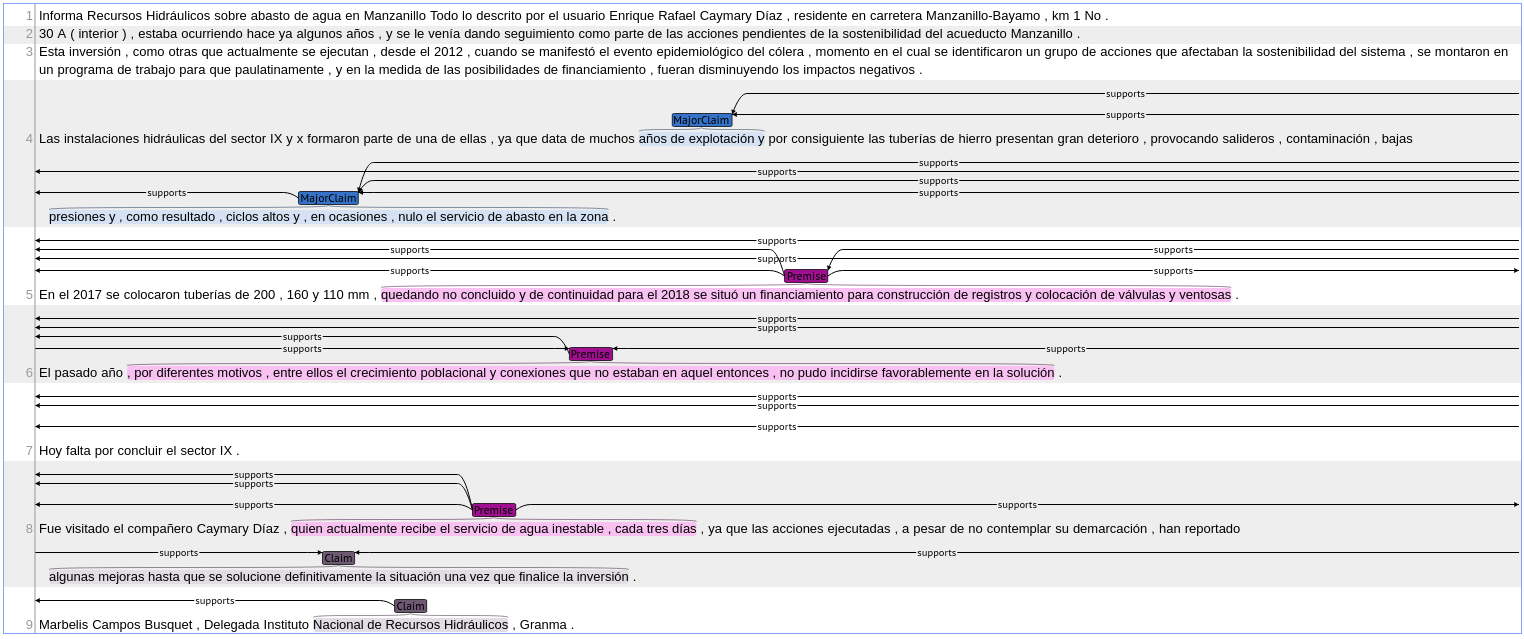
\includegraphics[scale=.4]{Graphics/persuasive_2019-01-25_informa-recursos-hidraulicos-sobre-abasto-de-agua-en-manzanillo_abasto-de-agua-en-manzanillo.png}
% 	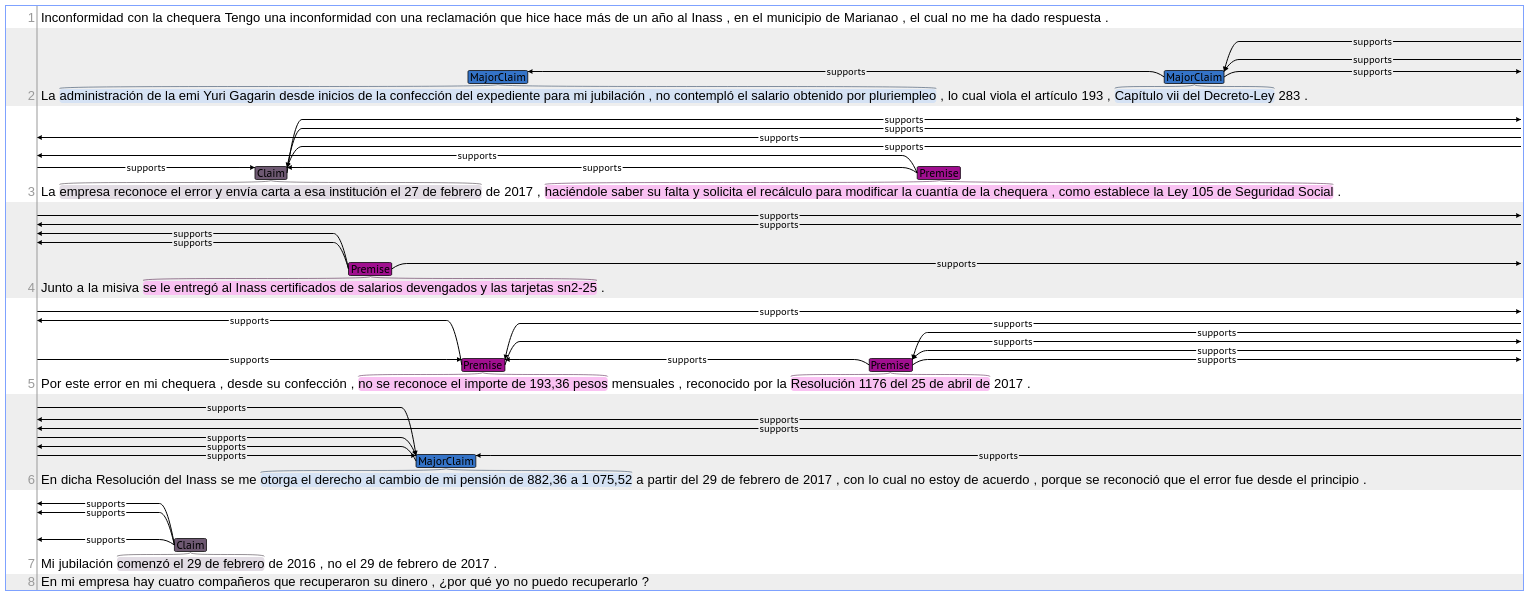
\includegraphics[width=7cm]{Graphics/persuasive_2019-03-22_inconformidad-con-la-chequera.png}
% 	\caption{Visualización con Brat de las estructuras argumentativas.}
% 	\label{fig:brat_persuasive_granma_letters}
% \end{figure}

% \subsection{Formato Estándar}

% El formato estándar creado es basado en el esquema de anotación CoNLL, donde se anotan a nivel de \textit{token} todos los aspectos 
% relevantes para las tareas a realizar. La segmentación de las UDAs son representadas por las anotaciones 
% BIO o BIOES en cada palabra, en adición, las clasificaciones de estas son anotadas al adicionar el nombre 
% de esta separada por un guión. Las relaciones son anotadas auxiliándose de la distancia argumentativa, estas 
% son agregadas al anotar el tipo de relación con su respectiva distancia ambas separadas por un guión. A 
% continuación se muestran ejemplos de este formato, conformado por el \textit{token}, su clasificación BIOES, su clasificación
% UDA, y las relaciones representadas por su clasificación y su distancia argumentativa:

% \begin{itemize}
% 	\item Elemento fuera de una UDA: $an\text{á}lisis \quad O$
% 	\item UDA intermedia con una relación: $contribuye \quad I-Premise-attacks-5$
% 	\item Inicio de UDA con dos relaciones: $atletas \quad B-Claim-attacks--1-attacks-12$
% \end{itemize}

\section{Resultados}

Para realizar la selección del modelo se utilizó el corpus de Ensayos Argumentativos. Con este se ajustaron
las arquitecturas e hiperparámetros de los modelos propuestos. La mejor combinación de estos fue utilizada 
para el entrenamiento de los corpus restantes. Finalmente, los modelos fueron utilizados para anotar los 
textos de la sección ``Cartas a la Dirección'' de \textit{Granma}. 

% \subsection{Hardware}

% Gran parte del procesamiento se llevo a cabo en una computadora $i5$ con $8GB$ de RAM ampliada con $4GB$ de memoria 
% \textit{swap} \cite{swap}, aunque se requirió el uso de la plataforma Colab \cite{colab} para 
% el entrenamiento de algunos modelos por falta de recursos locales.

\subsection{Segmentador de UDA}

% En el entrenamiento del segmentador de UDA se hicieron variaciones en la arquitectura propuesta con respecto a la
% presencia o no de las siguientes componentes, presentando cuatro candidatos (Tabla \ref{table:segmenter_architecture_table}):

% \begin{itemize}
% 	\item Atributos de POS en la entrada del algoritmo (POS).
% 	\item Atributos extraídos por la CNN de la palabra (Char-CNN).
% 	\item Atributos extraídos por la LSTM bidireccional de la palabra (Char-LSTM).
% 	\item Conexiones residuales (Res).
% 	\item Capa densa final (Densa).
% 	\item Capas de normalizaciones (Norm).
% \end{itemize}

% \begin{table}[h]
% 	\begin{center}
% 		\begin{tabular}{|l|c|c|c|c|} 
% 			\hline\rule{-2pt}{15pt}
% 			{\bf Modelos}  & {\bf 1}     & {\bf 2}     & {\bf 3}     & {\bf 4}     \\ 
% 			\hline\rule{-4pt}{10pt}
% 			POS 	  & $\times$  & $\times$ 	 & $\checkmark$ & $\checkmark$ \\
% 			Char-CNN  & $\times$  & $\checkmark$ & $\checkmark$ & $\checkmark$ \\
% 			Char-LSTM & $\times$  & $\checkmark$ & $\checkmark$ & $\checkmark$ \\
% 			Residual  & $\times$  & $\checkmark$ & $\checkmark$ & $\checkmark$ \\
% 			Norm 	  & $\times$  & $\checkmark$ & $\checkmark$ & $\checkmark$ \\
% 			Densa 	  & $\times$  & $\times$ 	 & $\times$ 	& $\checkmark$ \\
% 			\hline
% 		\end{tabular}
% 	\end{center}
% 	\caption{\label{table:segmenter_architecture_table}Variantes de arquitectura de los modelos de segmentación de UDA.}
% \end{table}

% En la Figura \ref{fig:segmenter_model_loss} se observan las diferentes curvas de aprendizaje de los modelos 
% probados. Se muestra la rápida convergencia de los modelos con conexiones residuales y normalizaciones.
% Se muestra también la tendencia al sobreajuste en el entrenamiento entre los pasos 17-20, en donde se detiene el 
% entrenamiento para evitar el crecimiento del error de generalización.

% \begin{figure}[h]
% 	\centering
% 	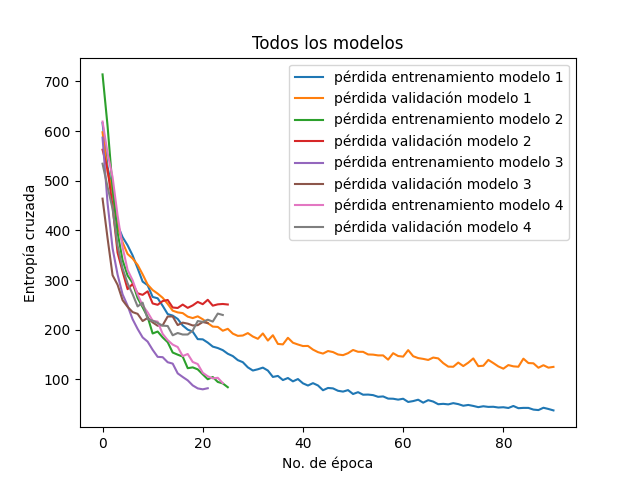
\includegraphics[width=7cm,clip]{Graphics/persuasive_essays_all_linked_crf_loss.png}
% 	\caption{Pérdida de los modelos segmentadores.}
% 	\label{fig:segmenter_model_loss}
% \end{figure}

% Las métricas 100\%F1 y 50\%F1 muestran que los modelos 1 y 2 presentan un desempeño menor que los 3 y 4. 
% Se muestra un ligero aumento de 1\% en las 50\%F1 en el modelo 4 con respecto 
% al modelo 3, aunque las métricas de F1 en el 3 superan a las de 4. Se considera a la 
% segmentación como tarea principal, por lo que se selecciona como mejor modelo al 4 (Figura \ref{fig:test_segmenter_model_metrics}).
% Las distinciones BIOES en los nombres de tablas o métricas constituyen las métricas correspondientes 
% a la segmentación estrictamente, mientras las que no poseen dicha distinción constituyen al proceso 
% conjunto de segmentación y clasificación de UDAs. 

% \begin{figure}[h]
% 	\centering
% 	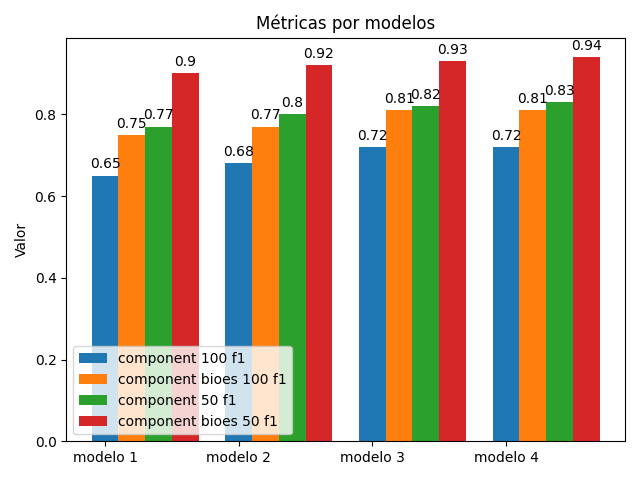
\includegraphics[width=7cm,clip]{Graphics/persuasive_essays_all_linked_components.png}
% 	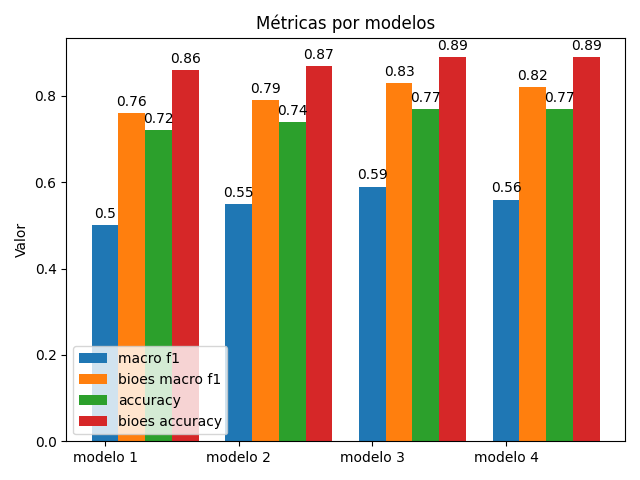
\includegraphics[width=7cm,clip]{Graphics/persuasive_essays_all_linked_macro_micro_metrics.png}
% 	\caption{Métricas del conjunto de pruebas de los modelos segmentadores.}
% 	\label{fig:test_segmenter_model_metrics}
% \end{figure}

El modelo seleccionado fue usado en el entrenamiento de los demás conjuntos de datos obteniendo los resultados mostrados
en Tabla \ref{table:test_metrics_segmenter} y Tabla \ref{table:test_bioes_metrics_segmenter}.

Las métricas 50\%F1 y 100\%F1 \cite{persing2016end} están
basadas en la idea de la métrica F1, pero orientada a secuencias, donde el número denota el porcentaje de secuencia inferida que debe coincidir con 
la secuencia anotada para ser considerado una coincidencia.

\begin{table}[h]
	\begin{center}
		\scalebox{0.7}{
		\begin{tabular}{|l|c|c|c|} 
			\hline\rule{-2pt}{15pt}
			{\bf Corpus}                 & {\bf Ensayos} 		& {\bf CDCP} & {\bf AbsTRCT} \\ 
						                 & {\bf Argumentativos} & 			 & 				 \\ 
			\hline\rule{-4pt}{10pt}
			F1 Ponderado 				 & 0,76         		& 0,65     	 & 0,86          \\
			Macro F1                     & 0,56         		& 0,45     	 & 0,50          \\
			\textit{Accuracy}            & 0,77         		& 0,66     	 & 0,87          \\ 
			100\%F1						 & 0,72         		& 0,61     	 & 0,61          \\ 
			50\%F1                		 & 0,83         		& 0,68     	 & 0,75          \\ 
			\hline
		\end{tabular}
		}
	\end{center}
	\caption{\label{table:test_metrics_segmenter}Métricas de las pruebas del segmentador de UDA.}
\end{table}
\begin{table}[h]
	\begin{center}
		\scalebox{0.7}{
		\begin{tabular}{|l|c|c|c|} 
			\hline\rule{-2pt}{15pt}
			{\bf Corpus}                 & {\bf Ensayos} 		& {\bf CDCP} & {\bf AbsTRCT} \\ 
						                 & {\bf Argumentativos} & 			 & 				 \\ 
			\hline\rule{-4pt}{10pt}
			F1 Ponderado 				 & 0,89         		& 0,95     	 & 0,90          \\
			Macro F1                     & 0,82         		& 0,56     	 & 0,79          \\
			\textit{Accuracy}            & 0,89         		& 0,96     	 & 0,91          \\ 
			100\%F1                		 & 0,81         		& 0,82     	 & 0,66          \\ 
			50\%F1                		 & 0,94         		& 0,93     	 & 0,82          \\ 
			\hline
		\end{tabular}
		}
	\end{center}
	\caption{\label{table:test_bioes_metrics_segmenter}Métricas BIOES de las pruebas del segmentador de UDA.}
\end{table}

En las tablas se observa una diferencia entre los valores de F1 Ponderado y 
de Macro F1, dadas por el pobre balance de las clases que hace que las menos
representadas sean más difíciles de ser correctamente anotadas. Los valores
mayores de 50\%F1 en comparación con 100\%F1 indican que el modelo logra 
inferir las posiciones de las UDA de manera general, pero sus límites se hacen 
más complejos de discernir. 

\subsection{Predictor de Enlaces}

Para el modelo se realizó un voto conjunto del ensamblado de tres modelos, dado que el entrenamiento 
está basado en la aleatoriedad, se entrenan los modelos con los mismos datos obteniendo inferencias no
necesariamente iguales.
% Para la selección del modelo se entrenaron diferentes variantes de arquitecturas e hiperparámetros, y 
% al igual que en el segmentador de UDAs se realizó la selección del modelo que mejor se desempeñó en 
% el conjunto de datos de Ensayos Argumentativos. De las variaciones surgieron las siguientes propuestas
% (Tabla \ref{table:link_predictor_architecture_table}):

% \begin{table}[h]
% 	\begin{center}
% 		\scalebox{0.9}{
% 		\begin{tabular}{|l|c|c|c|c|} 
% 			\hline\rule{-2pt}{15pt}
% 			{\bf Modelos}  		& {\bf 1}      & {\bf 2}  & {\bf 3} 	 & {\bf 4} 		\\ 
% 			\hline\rule{-4pt}{10pt}
% 			Atención 		    & $\times$     & $\times$ & $\checkmark$ & $\checkmark$ \\
% 			Pooling  		    & 5    		   & 10       & 1       	 & 1    		\\
% 			\textit{Dropout}    & 0,5   	   & 0,1      & 0,1       	 & 0,5	    	\\
% 			Tasa de 			&			   & 		  &		     	 & 		    	\\
% 			aprendizaje 		& 0,0015 	   & 0,003    & 0,003      	 & 0,0015    	\\
% 			Paciencia			& 10 		   & 5		  & 5       	 & 10		   	\\
% 			Devolver			&			   & 		  & 		  	 & 				\\
% 			mejores				& $\checkmark$ & $\times$ & $\times$  	 & $\checkmark$ \\
% 			\hline
% 		\end{tabular}
% 		}
% 	\end{center}
% 	\caption{\label{table:link_predictor_architecture_table}Variantes de arquitectura de los modelos de predicción de enlaces.}
% \end{table}

% Las curvas de aprendizaje del proceso de entrenamiento de los modelos (Figura \ref{fig:link_prediction_model_loss}) 
% muestran un nivel de sobreajuste 
% elevado que disminuyen cuando el \textit{dropout} aumenta. Además, se observan valores de pérdida elevados lo que significa 
% que al modelo le cuesta ajustarse de manera satisfactoria a los datos.

% \begin{figure}[h]
% 	\centering
% 	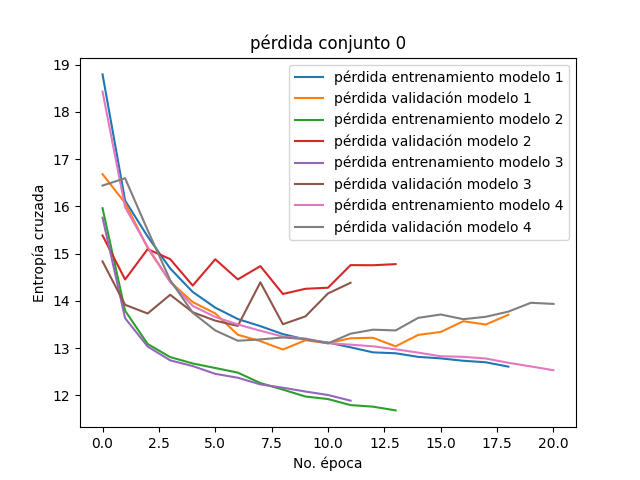
\includegraphics[width=7cm,clip]{Graphics/persuassive_essays_all_linked_link_prediction_loss_model_1.png}
% 	\caption{Curvas de aprendizaje de los modelos de predicción de enlaces.}
% 	\label{fig:link_prediction_model_loss}
% \end{figure}

% Las métricas obtenidas por las diferentes versiones de los modelos 
% (Figura \ref{fig:link_prediction_model_metrics}) 
% muestran que el modelo 2 constituye una opción ligeramente superior en lo correspondiente a 
% predicción de enlace a los otros modelos. Esos hiperparámetros
% fueron utilizados para el entrenamiento con los demás conjuntos de datos.

% \begin{figure}[h]
% 	\centering
% 	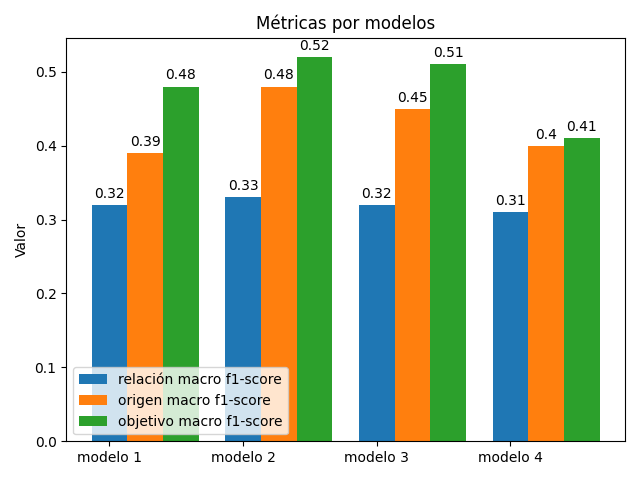
\includegraphics[width=7cm]{Graphics/persuasive_essays_all_linked_all_relation_f1_scores.png}\\
% 	\text{a)}\\
% 	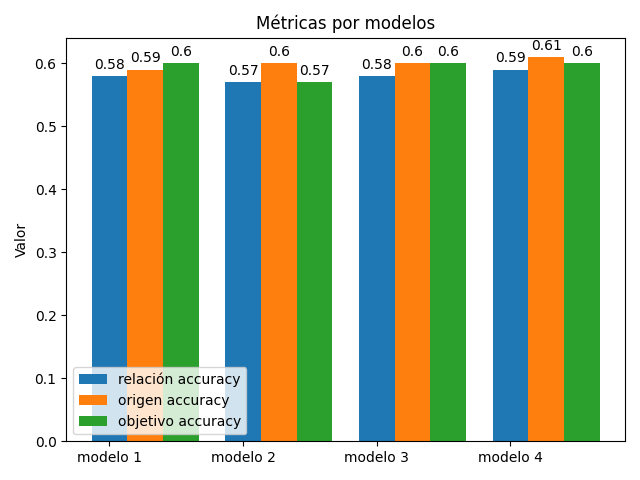
\includegraphics[width=7cm]{Graphics/persuasive_essays_all_linked_all_relation_accuracy.png}\\
% 	\text{b)}\\
% 	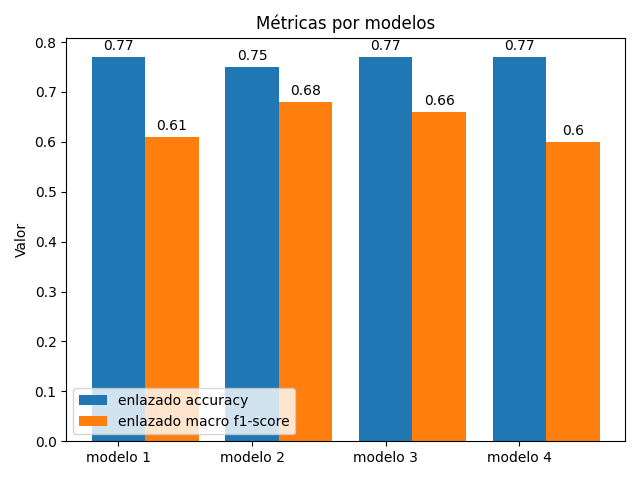
\includegraphics[width=7cm]{Graphics/persuasive_essays_all_linked_all_relation_linked.png}\\
% 	\text{c)}
% 	\caption{Métricas F1 de la clasificación de enlace (a), \textit{accuracy} (b) y
% 		F1 de la predicción de enlace (c) de los modelos de predicción de enlaces.}
% 	\label{fig:link_prediction_model_metrics}
% \end{figure}

En el entrenamiento del modelo en los demás conjuntos de datos se obtuvieron los resultados de las Tablas 
\ref{table:test_relation_metrics_link_predictor_relation_classification} y 
\ref{table:test_relation_metrics_link_predictor_link_prediction}.
% y \ref{table:test_source_metrics_link_predictor}.

\begin{table}[h]
	\begin{center}
		\begin{tabular}{|l|c|c|} 
			\hline\rule{-2pt}{15pt}
			{\bf Corpus}                 & {\bf Macro F1} & {\bf \textit{Accuracy}} \\
			\hline\rule{-4pt}{10pt}
			Ensayos				 		 & 				  & 						\\ 
			argumentativos 		 		 & 0,33			  & 0,57					\\ 
			CDCP                   		 & 0,37			  & 0,63					\\ 
			AbsTRCT               		 & 0,39			  & 0,61					\\ 
			\hline
		\end{tabular}
	\end{center}
	\caption{\label{table:test_relation_metrics_link_predictor_relation_classification}Métricas de clasificación de relaciones de las pruebas del predictor de enlace.}
\end{table}

\begin{table}[h]
	\begin{center}
		\begin{tabular}{|l|c|c|} 
			\hline\rule{-2pt}{15pt}
			{\bf Corpus}                 & {\bf Macro F1}  & {\bf \textit{Accuracy}} \\
			\hline\rule{-4pt}{10pt}
			Ensayos 			 		 & 	               & 	                    \\ 
			argumentativos 				 & 0,68            & 0,75                   \\ 
			CDCP                   		 & 0,79            & 0,68                   \\ 
			AbsTRCT               		 & 0,83            & 0,74                   \\ 
			\hline
		\end{tabular}
	\end{center}
	\caption{\label{table:test_relation_metrics_link_predictor_link_prediction}Métricas de predicción de relaciones de las pruebas del predictor de enlace.}
\end{table}

En la Tabla \ref{table:test_relation_metrics_link_predictor_relation_classification} se observan
valores más discretos que en la Tabla \ref{table:test_relation_metrics_link_predictor_link_prediction}
en ambas métricas. Esta diferencia en la métrica Macro F1 se interpreta como el fallo del modelo 
en predecir correctamente la clase de la relación. En la tarea de predicción de 
enlace el modelo se desempeña mejor, aunque con diferencias entre los conjuntos de datos, 
dando a entender que la estructura de las relaciones de estos pueden influir en el resultado.

% \begin{table}[h]
% 	\begin{center}
% 		\begin{tabular}{|l|c|c|c|} 
% 			\hline\rule{-2pt}{15pt}
% 			{\bf Corpus}                 & {\bf F1 Macro} & {\bf \textit{Accuracy}} \\ 
% 			\hline\rule{-4pt}{10pt}
% 			Ensayos				   & 	      & 	            \\ 
% 			argumentativos		   & 0,48     & 0,60            \\ 
% 			CDCP                   & 0,26     & 0,52            \\ 
% 			AbsTRCT                & 0,51     & 0,79            \\ 
% 			\hline
% 		\end{tabular}
% 	\end{center}
% 	\caption{\label{table:test_source_metrics_link_predictor}Métricas de predicción de fuente de las pruebas del predictor de enlace.}
% \end{table}

% \begin{table}[h]
% 	\begin{center}
% 		\begin{tabular}{|l|c|c|c|} 
% 			\hline\rule{-2pt}{15pt}
% 			{\bf Corpus}           & {\bf Macro F1} & {\bf \textit{Accuracy}} \\ 
% 			\hline\rule{-4pt}{10pt}
% 			Ensayos				   & 	      & 	            \\
% 			argumentativos 		   & 0,52     & 0,57            \\
% 			CDCP                   & 0,36     & 0,54            \\
% 			AbsTRCT                & 0,53     & 0,81            \\ 
% 			\hline
% 		\end{tabular}
% 	\end{center}
% 	\caption{\label{table:test_target_metrics_link_predictor}Métricas de predicción de objetivo de las pruebas del predictor de enlace.}
% \end{table}

% \subsection{Acoplamiento de los modelos}

% Dado que la clasificación de UDAs es hecha tanto en el segmentador como en el predictor de enlaces, es necesaria 
% la selección de cómo se va a desambiguar esta clasificación. En caso de seleccionar el predictor de enlaces como 
% clasificador final, surgen varias cuestiones, como por ejemplo, que las UDAs pueden tomar varias clasificaciones o el
% predictor no toma el contexto del texto completo en la clasificación. Aunque la primera puede ser corregida
% mediante la selección de la clase más votada o algún otro criterio, la segunda presenta un mayor problema. Por
% esto es seleccionada la clasificación del segmentador como etiqueta final para las UDAs y el predictor es usado para 
% la tarea de extracción y clasificación de relaciones.

\section{Evaluación cualitativa de la EA}

Dado que las estructuras argumentativas varían en su forma en cada corpus es complejo realizar un método que evalúe de forma 
justa los resultados obtenidos por los diferentes modelos de manera conjunta. Una variante sería anotar las cartas 
con los esquemas argumentativos presentes en los conjuntos de datos, esto constituye una labor en la que se requiere
personal experto, previo estudio y preparación, además de tiempo. 

Por ello, el proceso que se llevó a cabo en esta investigación para realizar la 
validación consistió en un análisis cualitativo realizado a criterio del autor. Para esto se seleccionaron 15 pares 
de cartas, la carta original y la respuesta enviada a esta. Cada una de estas 30 cartas fueron anotadas por los modelos entrenados en cada 
conjunto de datos y se realizó una evaluación que consideró si la UDA se extrajo y clasificó correctamente, 
así como si la relación también fue extraída y clasificada por el modelo de manera adecuada.

% \begin{itemize}
% 	\item Muchos falsos positivos en la predicción de enlaces, debido a la manera en la manera componente a componente que 
% 	se hacen
% 	\item En los textos en donde la segmentación es por oraciones, los puntos relacionados a otra acción que 
% 	no sea separar oraciones son seleccionados como separadores.
% 	\item La segmentación, se queda corta o larga?
% \end{itemize}

\subsection{Análisis del corpus Ensayos Argumentativos}

% \begin{figure}[h!]
% 	\begin{center}
% 		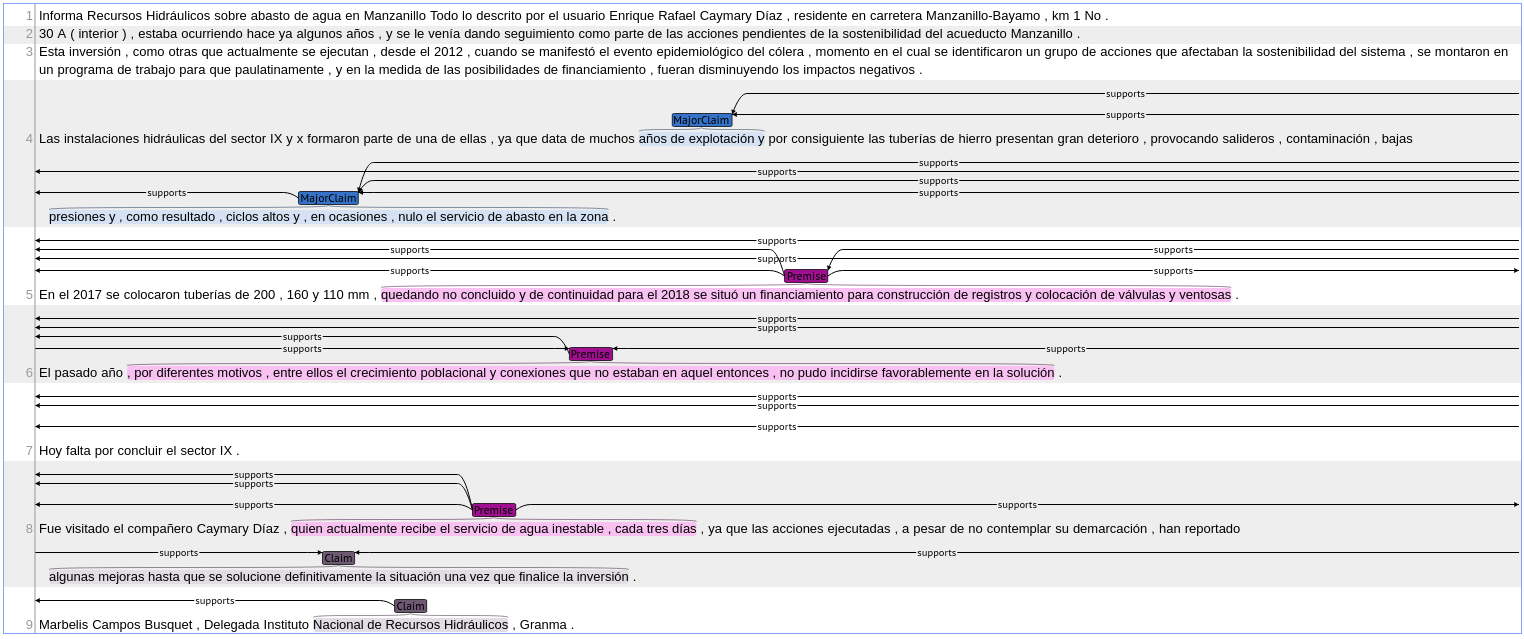
\includegraphics[scale=.4]{Graphics/persuasive_2019-01-25_informa-recursos-hidraulicos-sobre-abasto-de-agua-en-manzanillo_abasto-de-agua-en-manzanillo.png}
% 		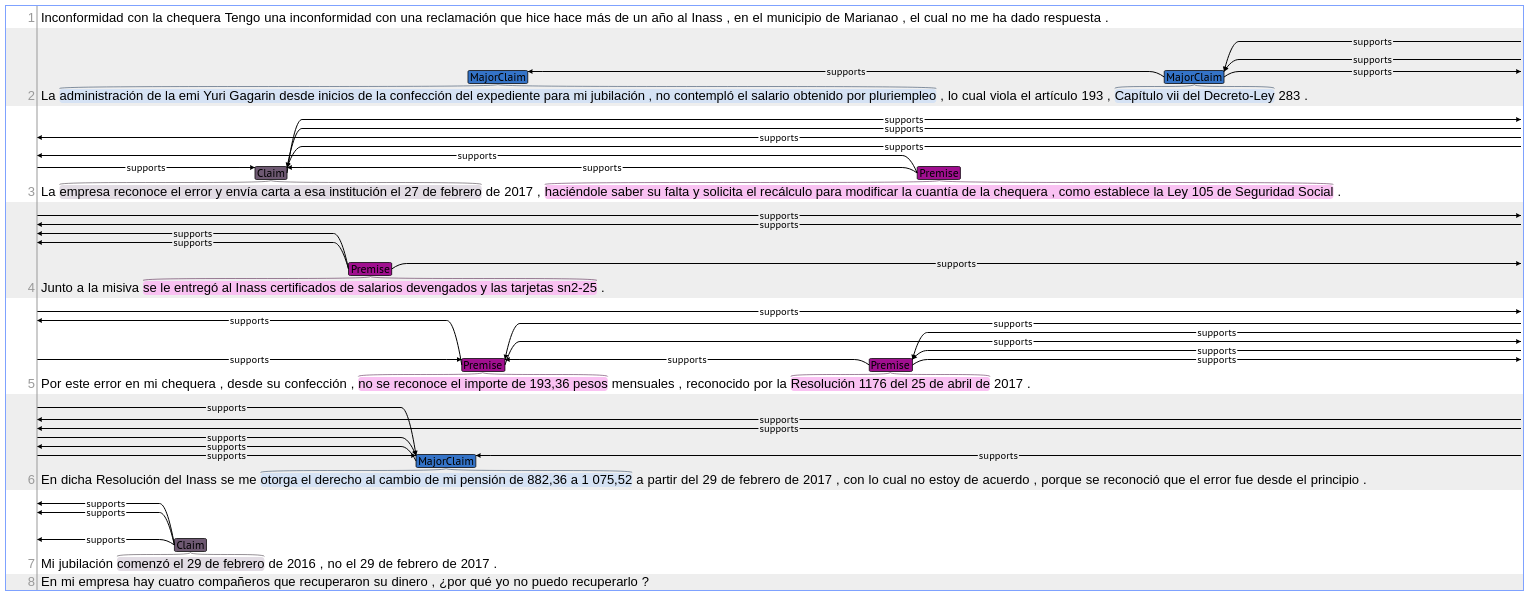
\includegraphics[scale=.4]{Graphics/persuasive_2019-03-22_inconformidad-con-la-chequera.png}
% 	    \caption{A}\label{fig:persuasive_granma_letters}
% 	\end{center}
% \end{figure}

Los ensayos argumentativos presentan una anotación de UDAs a un nivel de unidades de texto que pueden ser 
más pequeñas que oraciones y clasifican estas en las clases \textit{MajorClaim} (MC), \textit{Claim} (C) y \textit{Premise}
(P). Las relaciones se clasifican en de \textit{supports} y \textit{attacks}. 

En general, se observan problemas en la segmentación de UDAs debido al formato y dominio del texto.
Las cartas presentan una estrutura donde al final se realiza una firma poniendo información acerca del remitente.
Esta estructura no contribuye a la argumentación, pero el modelo en varias ocasiones detecta componentes en estas. 
Otro problema se observa en la extracción de supuestas UDAs sin componente argumentativo,
generalmente, estos elementos, si se expanden, pueden lograr establecer una mejor UDA.

Ejemplos donde el modelo propuesto no fue exitoso:
\begin{itemize}
	% \item \text{} [años de explotación y]$_{MC}$
	%       : muy corto y no informativo. % 2019-01-25_informa-recursos-hidraulicos-sobre-abasto-de-agua-en-manzanillo_abasto-de-agua-en-manzanillo.txt.conll.link.conll.ann
	\item \text{} [en cada uno de los establecimientos de nuestra Cadena de Tiendas]$_{MC}$
	      : incompleto, mejora incorporando elementos de la izquierda (No a todos los productos con próxima fecha de vencimiento se le aplica rebaja de precios). % 2018-12-07_responde-trd-caribe-al-consumidor_a-proposito-de-la-proteccion-al-consumidor.txt.conll.link.conll.ann
	% \item \text{} [Director División Grandes Centros]$_{MC}$ [TRD Caribe]$_{C}$
	%       : mala clasificación y segmentación. %  2018-12-07_responde-trd-caribe-al-consumidor_a-proposito-de-la-proteccion-al-consumidor.txt.conll.link.conll.ann
	\item \text{} [Esperamos lo antes posible una solución]$_{P}$
	      : en contexto, no contiene información que lo haga premisa. % 2018-10-05_abasto-de-agua-en-manzanillo.txt.conll.link.conll.ann
	% \item \text{} [no podemos permitir]$_{C}$
	%       : no establece una \textit{claim}. % 2017-06-30_inass-reconoce-razon-de-ramiro-castellanos-por-inconformidad-con-trato-de-especialista-de-las-tunas_pregunta-quien-le-paga-su-jubilacion.txt.conll.link.conll.ann
\end{itemize}

Ejemplos donde el modelo fue exitoso:
\begin{itemize}
	% \item \text{} [no se le puede volver a despachar, tiene que ver a la administración (si está ahí en ese momento),
	% 	      si no, regresar al día siguiente para que se le acredite lo sucedido]$_{MC}$ % 2021-02-26_inconvenientes-con-tarjetas-de-combustible-en-moneda-nacional.txt.conll.link.conll.ann
	% \item \text{} [administración de la EMI Yuri Gagarin desde inicios de la confección del expediente para
	% 	      mi jubilación, no contempló el salario obtenido por pluriempleo]$_{MC}$ % 2019-03-22_inconformidad-con-la-chequera.txt.conll.link.conll.ann
	\item pudiese [contribuir al ahorro de agua y la prestación de un mejor servicio]$_C$ % 2018-10-05_abasto-de-agua-en-manzanillo.txt.conll.link.conll.ann
	\item \text{} [es que estamos limitados de este servicio, y no desde hace un tiempo, es que nunca lo hemos tenido]$_P$ % 2018-05-18_sin-cobertura-en-guara-mayabeque.txt.conll.link.conll.ann
	% \item \text{} [el número de carné de identidad que se encontraba en dicha base de datos correspondía a otra persona que
	% 	      fue reportada como fallecida]$_P$ % 2017-06-30_inass-reconoce-razon-de-ramiro-castellanos-por-inconformidad-con-trato-de-especialista-de-las-tunas_pregunta-quien-le-paga-su-jubilacion.txt.conll.link.conll.ann
\end{itemize}

Las relaciones anotadas por el modelo tienden a contener falsos positivos, además
dado que este conjunto de datos posee un gran desbalance en las etiquetas de las relaciones favoreciendo 
estas a las de \textit{supports}, el modelo no fue capaz de realizar anotaciones de \textit{attacks}, tanto en 
el conjunto de pruebas como en las ``Cartas a la Dirección'' del \textit{Granma}.

\subsection{Análisis de CDCP}

% \begin{figure}[h!]
% 	\begin{center}
% 		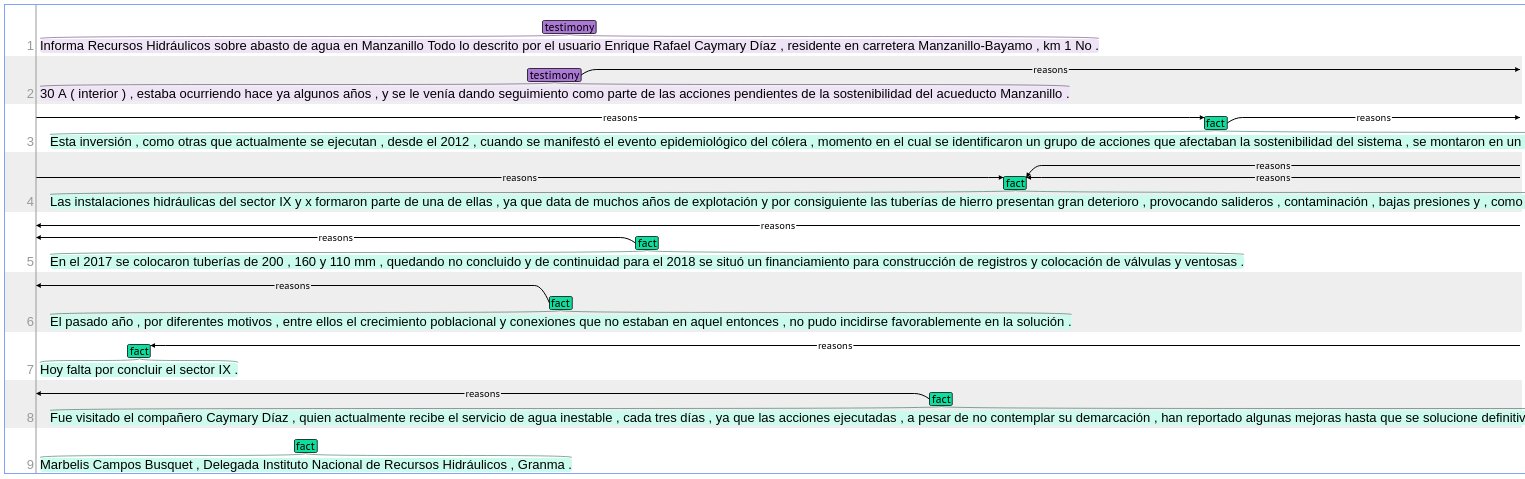
\includegraphics[scale=.4]{Graphics/cdcp_2019-01-25_informa-recursos-hidraulicos-sobre-abasto-de-agua-en-manzanillo_abasto-de-agua-en-manzanillo.png}
% 		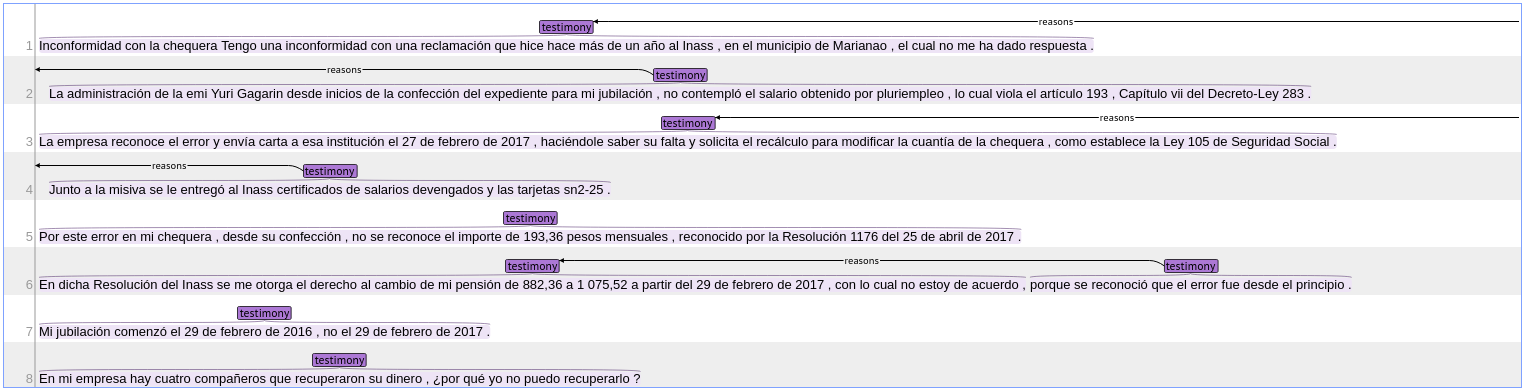
\includegraphics[scale=.4]{Graphics/cdcp_2019-03-22_inconformidad-con-la-chequera.png}
% 	    \caption{A}\label{fig:cdcp_granma_letters}
% 	\end{center}
% \end{figure}

El corpus CDCP las UDAs son segmentadas, en la mayoría de los casos, en oraciones 
(solamente el 1\% de los \textit{tokens} se encuentran fuera de una UDA),
estas son clasificadas en \textit{testimony} (T), \textit{fact} (F), \textit{policy} (P), \textit{reference} (R)
y \textit{value} (V). Las relaciones presentan dos tipos de relaciones \textit{evidences} y \textit{reasons}.

Los errores más comunes cometidos por el modelo propuesto en la segmentación, provienen del uso 
de signos de puntuación que no representan un cambio de oración, en estos casos se separan las UDAs. También
existen errores de clasificación incorrecta, de, por ejemplo, \textit{testimony} que podrían ser \textit{fact}.

Ejemplos deonde el modelo propuesto no fue exitoso:
\begin{itemize}
	% \item \text{} [\dots Bayamo, km 1 No.]$_T$ [30 A (interior), \dots]$_T$
	%       : uso del \textbf{.} para abreviar número se toma como separador de UDA. % 2019-01-25_informa-recursos-hidraulicos-sobre-abasto-de-agua-en-manzanillo_abasto-de-agua-en-manzanillo.txt.conll.link.conll.ann
	% \item \text{} [\dots ,desde el 1ro.]$_T$ [de marzo \dots]$_T$
	%       : Uso del \textbf{.} para abreviar primero se toma como separador de UDA. % 2019-05-24_le-retribuyen-la-diferencia-reclamada-de-su-pension_inconformidad-con-la-chequera.txt.conll.link.conll.ann
	\item \text{} [Junto a la misiva se le entregó al Inass certificados de salarios devengados y las tarjetas sn2-25.]$_T$
	      : se clasifica mejor como \textit{fact}. % 2019-03-22_inconformidad-con-la-chequera.txt.conll.link.conll.ann
	\item \text{} [Caridad Real Gutiérrez, Jefe de Trámites y Pensiones, Inass.]$_T$
	      : firma de la carta como elemento argumentaivo. % 2019-05-24_le-retribuyen-la-diferencia-reclamada-de-su-pension_inconformidad-con-la-chequera.txt.conll.link.conll.ann
\end{itemize}

Ejemplos donde el modelo propuesto fue exitoso:
\begin{itemize}
	% \item \text{} [En el 2017 se colocaron tuberías de 200, 160 y 110 mm, quedando no concluido y de
	% 	      continuidad para el 2018 se situó un financiamiento para construcción de registros y colocación de 
	% 	      válvulas y ventosas.]$_F$ % 2019-01-25_informa-recursos-hidraulicos-sobre-abasto-de-agua-en-manzanillo_abasto-de-agua-en-manzanillo.txt.conll.link.conll.ann
	\item \text{} [Mi jubilación comenzó el 29 de febrero de 2016, no el 29 de febrero de 2017.]$_T$ % 2019-03-22_inconformidad-con-la-chequera.txt.conll.link.conll.ann
	\item \text{} [No se sabe cuánto queda, lo que obliga al cliente a estar haciendo cuentas constantemente.]$_F$ % 2021-05-07_servicentros-operan-diversos-medios-de-pago-electronicos_inconvenientes-con-tarjetas-de-combustible-en-moneda-nacional.txt.conll.link.conll.ann
\end{itemize}

La cantidad de relaciones anotadas por el modelo entrenado en este corpus
disminuye en comparación a las anotadas por el modelo entrenado con el corpus Ensayos
Argumentativos. Las relaciones \textit{reasons} son las más encontradas. % TODO Poner numeros de esto

% Las relaciones presentes disminuyen en cantidad en comparación con lo visto en los textos anotados con el modelo 
% entrenado con Ensayos Argumentativos. Prevaleciendo las relaciones de \textit{reasons}. A consideración del autor,
% la cantidad de los falsos positivos son menores que cuando se utilizó el modelo entrenado con el corpus Ensayos Argumentativos.

\subsection{Análisis del corpus AbsTRCT}

% \begin{figure}[h!]
% 	\begin{center}
% 		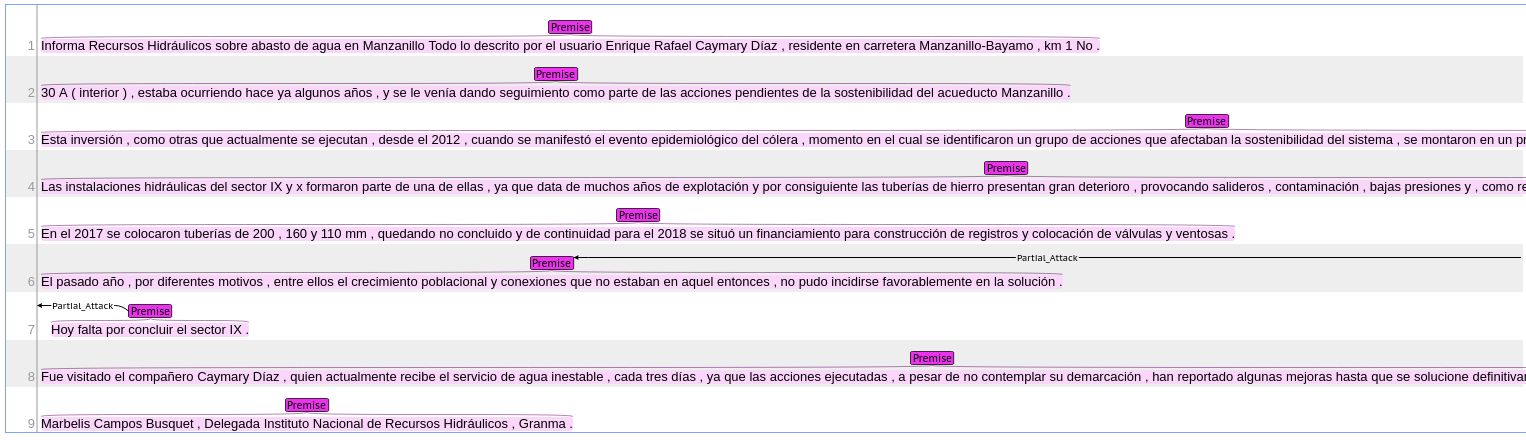
\includegraphics[scale=.4]{Graphics/abstrct_2019-01-25_informa-recursos-hidraulicos-sobre-abasto-de-agua-en-manzanillo_abasto-de-agua-en-manzanillo.png}
% 		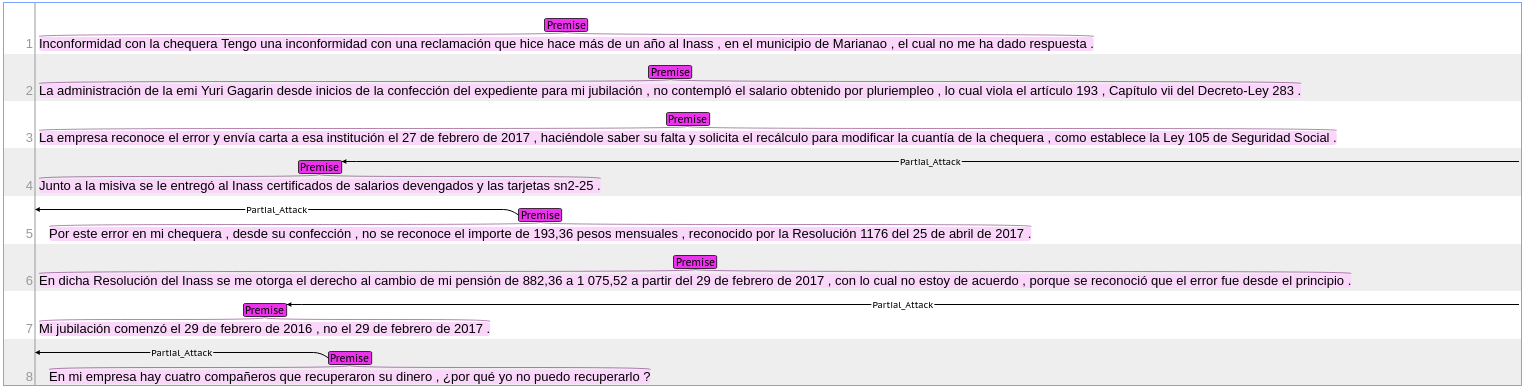
\includegraphics[scale=.4]{Graphics/abstrct_2019-03-22_inconformidad-con-la-chequera.png}
% 		\caption{A}\label{fig:abstrct_granma_letters}
% 	\end{center}
% \end{figure}

El conjunto de datos presenta un estilo de segmentación de UDAs en donde se anotan 
secciones de textos más grandes que en el corpus Ensayos Argumentativos, aunque no necesariamente 
todas las oraciones o la oración completa es considerada argumentativa. 
Estas se clasifican igual que el corpus Ensayos Argumentativos, aunque 
en este conjunto de datos se presenta un desbalance de etiquetas grande, favoreciendo 
a las \textit{Premise} y las \textit{Claim}, % TODO Poner porcientos
dejando sin representación casi a \textit{MajorClaim}
(menor del 1\% de las etiquetas BIOES), lo que trajo como consecuencia que el modelo no fuera 
capaz de diferenciar este tipo de UDA. Las relaciones se presentaron como \textit{partial-attack},
\textit{attack} y \textit{support}, influenciadas también por la poca cantidad de relaciones de \textit{attack}.

En la clasificación de UDAs se evidencia una gran cantidad de \textit{Premise}.

Ejemplos deonde el modelo propuesto no fue exitoso:
\begin{itemize}
	% \item \text{} [\dots Calle 14, apto.]$_P$ [4 entre Zapata y 23, \dots]$_T$
	%       : uso del \textbf{.} para abreviar la palabra apartamento, que se toma como separador de UDA. % 2017-07-07_parque-en-pleno-deterioro-en-plaza.txt.conll.link.conll.ann
	\item \text{} [, Director División Grandes Centros TRD Caribe.]$_C$
	      : mala clasificación con mala segmentación y detección de \textit{claim} en pie de firma de la carta. 
\end{itemize}

Ejemplos donde el modelo propuesto fue exitoso:
\begin{itemize}
	% \item \text{} [Esta situación pudo haberse evitado y no podemos permitir que hechos como este ocurran pues,
	% 	      empañan la imagen de la institución que está destinada a brindar un servicio con calidad a la población en 
	% 	      general y en especial a los jubilados y pensionados.]$_P$ % 2017-06-30_inass-reconoce-razon-de-ramiro-castellanos-por-inconformidad-con-trato-de-especialista-de-las-tunas_pregunta-quien-le-paga-su-jubilacion.txt.conll.link.conll.ann
	\item \text{} [Esta respuesta considera sin razón la preocupación de un lector,
		      ¿así debe terminar la inquietud de un ciudadano, que confía en las instituciones con que cuenta la 
		      sociedad para enfrentar sus problemas?]$_C$ % 2017-05-12_cimex-se-dirige-a-limitado-fisico-motor_llamado-a-evaluar-situacion-de-piezas-y-baterias-para-equipos-motorizados-de-discapacitados.txt.conll.link.conll.ann
\end{itemize}

La cantidad de relaciones anotadas por el modelo entrenado en este corpus es la menor
de los demás conjuntos de datos. Se observa una gran cantidad de relaciones \textit{support}. % TODO Poner numeros de esto
Las relaciones clasificadas como \textit{partial-attack}, a consideración del autor, presentaron 
una baja precisión.

% Las relaciones tienen la menor cantidad de elementos de los otros conjuntos de datos, proliferando
% las relaciones de \textit{support}. En las clasificadas como \textit{partial-attack} se evidenció, a 
% consideración del autor, una baja precisión. 
% Por ejemplo 
% 	[\textit{cierto que la responsabilidad es de todos, pero la institucional es de la Dirección de Comunales.}]
% ataca a [\textit{Antonio Blanco, Director de Servicios Comunales Plaza,}].

\section{Discusión}

% \subsection{Comparación con el estado del arte}

Las comparaciones con el estado del arte se realizan por cada conjunto de datos y se muestran las 
métricas indicadas por los autores de cada propuesta. Cada corpus y propuesta 
presenta características únicas que hacen que difícil la comparación. 

Una de las principales dificultades está dada por el hecho de que las métricas calculadas son de la versión proyectada
al español, lo cual contribuye a variaciones en las etiquetas finales debido al lenguaje mismo 
o a errores en el proceso. Otros ejemplos en la dificultad de comparar las métricas se encuentra
en los enfoques tomados por las investigaciones anteriores a la hora de realizar las tareas.
En algunos casos la segmentación se presenta como una tarea de clasificación BIO, o
se separan por oraciones y las clasifican en argumentativas o no.

En el aspecto de clasificación
de las UDAs se emplean métodos como su clasificación independiente luego de ser extraída o su modelación
conjunta con la segmentación. En la extracción y clasificación de relaciones se observan técnicas de 
optimización de problemas enteros, clasificación por SVM o también probando los posibles enlaces dos 
a dos independientemente.

En la comparación de métodos se seleccionaron seis métricas que evalúan las diferentes 
tareas de la EA. La métrica BIOES F1 se refiere 
a la Macro F1 de la clasificación de las etiquetas BIOES, esta constituye una medida
que califica la tarea de segmentación de UDAs en el texto. 

La métrica Clas UDA F1 es 
calculada como la Macro F1 de las etiquetas BIOES junto con las etiquetas del tipo de 
UDA, medida que evalúa la tarea de clasificación de las UDAs. 

Rel Pred F1 es la medida 
Macro F1 de la predicción de enlaces y Rel Clas F1 la de la clasificación, estas 
son calculadas tomando en cuenta todos los pares seleccionados para el conjunto de 
datos. 

En las Tablas \ref{table:comparative_test_essays_f1_metrics_segmenter}-\ref{table:comparative_test_abstrct_f1_metrics_segmenter} el símbolo $\checkmark$ significa 
que los algoritmos son directamente comparables, el símbolo
$*$ expresa que el método de comparación es el mismo, pero no son usados los mismos 
elementos para calcular la métrica, y el símbolo $\times$ denota que la métrica no 
se computó en las investigaciones donde se propusieron los modelos.

\begin{table}[h]
	\begin{center}
		\scalebox{0.65}{
		\begin{tabular}{|p{30mm}|c|c|c|c|} 
			\hline\rule{-2pt}{15pt}
			{\bf Modelo}      				& {\bf BIOES} 			 & {\bf Clas} 	& {\bf Rel} 	& {\bf Rel} 	\\ 
						      				& {\bf F1} 				 & {\bf UDA F1} & {\bf Pred F1} & {\bf Clas F1} \\ 
			\hline\rule{-4pt}{10pt}
			Propuesto    					& 0,82     				 & 0,56      	& 0,68          & 0,33              \\
			\namecite{stab2017parsing} 		& 0,85  $\checkmark$     & 0,82      	& 0,58          & 0,70              \\
			\namecite{niculae2017argument}  & $\times$   			 & 0,77      	& 0,60          & $\times$          \\
			\namecite{galassi2021deep}      & $\times$  			 & 0,53      	& 0,36 *        & 0,18 *            \\ 
			\hline
		\end{tabular}
		}
		\caption{\label{table:comparative_test_essays_f1_metrics_segmenter}Métricas comparativas del corpus Ensayos Persuasivos.}
	\end{center}
\end{table}
\begin{table}[h]
	\begin{center}
		\scalebox{0.65}{
		\begin{tabular}{|p{30mm}|c|c|c|c|} 
			\hline\rule{-2pt}{15pt}
			{\bf Modelo}      				& {\bf BIOES} 			 & {\bf Clas} 	& {\bf Rel} 	& {\bf Rel} 	\\ 
						      				& {\bf F1} 				 & {\bf UDA F1} & {\bf Pred F1} & {\bf Clas F1} \\ 
			\hline\rule{-4pt}{10pt}
			Propuesto    				& 0,56      	 & 0,45         	 & 0,68 			 & 0,37               \\
			\cite{niculae2017argument}  & $\times$       & 0,73              & 0,27 			 &  $\times$          \\
			\cite{galassi2021deep} 		& $\times$  	 & 0,79              & 0,30	*   		 &  0,15	*         \\
			\hline
		\end{tabular}
		}
		\caption{\label{table:comparative_test_cdcp_f1_metrics_segmenter}Métricas comparativas del corpus CDCP.}
	\end{center}
\end{table}
\begin{table}[h]
	\begin{center}
		\scalebox{0.65}{
		\begin{tabular}{|p{30mm}|c|c|c|c|} 
			\hline\rule{-2pt}{15pt}
			{\bf Modelo}      				& {\bf BIOES} 			 & {\bf Clas} 	& {\bf Rel} 	& {\bf Rel} 	\\ 
												& {\bf F1} 				 & {\bf UDA F1} & {\bf Pred F1} & {\bf Clas F1} \\ 
			\hline\rule{-4pt}{10pt}
			Propuesto    				& 0,79      	 & 0,50              & 0,74 			 & 0,39               \\
			\cite{mayer2020transformer} & $\times$       & 0,88	$\checkmark$ & $\times$  		 & 0,66 *             \\
			\cite{galassi2021deep} 		& $\times$  	 & 0,91 	         & 0,54 *            & 0,70 *    		  \\
			\hline
		\end{tabular}
		}
		\caption{\label{table:comparative_test_abstrct_f1_metrics_segmenter}Métricas comparativas del corpus AbsTRCT.}
	\end{center}
\end{table}

% \subsection{Análisis de los conjuntos de datos}

Se considera que el corpus CDCP se ajusta mejor a las características de las ``Cartas 
a la Dirección''. Este presenta orígenes similares y un conjunto de etiquetas de UDAs que se ajustan más a lo observado 
en las Cartas. También las Cartas presentan un alto contenido argumentativo, por lo que marcar 
todas las oraciones como argumentativas no constituye una fuente grande de errores.
% , aunque esta parte puede ser mejorada

Una desventaja de este esquema sobre otros es la carencia de una 
clasificación de las relaciones que implique un ataque, aunque esto se cubre con el hecho de 
que en los conjuntos en donde existen estas, los resultados son pobres en ese aspecto. La cantidad 
y calidad de relaciones, aunque tiene espacio para mejorar, es aceptable dada la dificultad 
del problema en EA.

La ventaja del modelo entrenado con el corpus de Ensayos Argumentativos en la extracción 
y clasificación de UDA es que utiliza un conjunto de etiquetas que 
podría considerarse universal en la argumentación y además reduce el espacio de búsqueda de 
oraciones a segmentos de palabras, aunque estos puedan estar sujetos a errores. 

La versión del modelo propuesto entrenado sobre el corpus AbsTRCT constituye el modelo 
con menor rendimiento. La clasificación
de UDAs presentó una gran desproporción hacia \textit{Premise} dejando muchas \textit{Claim} % TODO Poner numeros
sin ser correctamente clasificadas. Sobre las relaciones, reportó un nivel muy bajo de 
relaciones por documento, respecto a las que se podrían formar.

\section{Conclusiones}

En la investigación se logró la extracción de estructuras argumentativas en los textos de las 
``Cartas a la Dirección'' del periódico \textit{Granma}. Para esto se hizo un análisis de los
modelos entrenado con los distintos conjuntos de datos y se seleccionó el modelo que más se ajustaba
al dominio de las cartas. Esta
selección se realizó sin tener un conjunto anotado por lingüistas de las Cartas,
por lo que los autores fueron los que establecieron los criterios cualitativos 
para la selección del modelo final.

En los resultados obtenidos en las tareas de segmentación y clasificación de UDAs se observan
valores 50\%F1 entre 0,82 y 0,94 y 0,68 y 0,83, respectivamente, indicando una segmentación aceptable 
pero que en ocasiones falla a la hora de clasificar correctamente. Al predecir los enlaces y clasificarlos 
los modelos obtienen resultados de Macro F1 entre 0,68 y 0,83 y 0,33 y 0,39, respectivamente. Estos evidencian
una mayor dificultad a la hora de trabajar con las relaciones, sobre todo al clasificarlas. 
Las comparaciones con las investigaciones previas con los resultados de los modelos entrenados 
se vieron dificultadas por los diferentes enfoques presentados en estas a la hora de seleccionar 
cómo modelar el problema y cómo procesar los datos para entrenar los modelos.

Este trabajo aportó nuevos conjuntos de datos, estos son las ``Cartas a la Dirección'' extraídas del \textit{Granma},
los corpus proyectados al español de Ensayos Argumentativos, AbsTRCT y CDCP y las Cartas 
anotadas con las estructuras argumentativas del modelo entrenado con el conjunto de datos CDCP. También
presentó unos modelos capaces de adaptarse a los diferentes esquemas que se puedan presentar en la argumentación,
haciéndolos viables para un estudio directo y sin el agrego de conocimiento específico de los datos.
% , evidenciado en el análisis hecho con tres conjuntos de datos independientes.

% En el trabajo se logró la extracción de estructuras argumentativas en los textos de las 
% ``Cartas a la Dirección'' del periódico \textit{Granma}. Para esto se 
% extrajeron los textos de las Cartas creando un conjunto de datos con estos y también
% se obtuvo las versiones proyectadas al español de Ensayos Argumentativos, AbsTRCT y CDCP.
% conteniendo, no solo el texto de las cartas, si no, los comentarios 
% escritos por los usuarios e información sobre la carta a la que responde, si es una respuesta.
% Se creó un software\footnote{\url{https://github.com/luisoibarra/argument-mining}} que puede 
% ser utilizado no solo para el trabajo con las Cartas a la Dirección, si no
% que este permite un uso general para las tareas de proyección de corpus y trabajo relacionados a la EA.
% Este permite incorporar nuevas componentes haciendo posible una extensión simple y desacoplada. 
% Los modelos creados, uno encargado 
% de la segmentación y clasificación de las UDAs, y otro de la extracción y clasificación de las 
% relaciones entre estas, fueron utilizados para la anotación de los textos extraídos. Estos modelos
% permiten el análisis de diferentes esquemas de anotación en los conjuntos de datos debido a su 
% Los resultados obtenidos en la tarea de segmentación se encuentran al nivel del estado del arte,
% en las demás tareas no se encontraron comparaciones directas al enfoque tomado en la propuesta,
% aunque no teniendo en cuenta esto, se obtienen comparativas inferiores en la clasificación
% de UDAs y en la clasificación de relaciones, aunque se supera la métrica de predicción de enlace. 
% Los resultados obtenidos del procesamiento de las ``Cartas a la Dirección'' son considerados 
% aceptables por autor.

El software implementado y los datos pueden encontrarse en \url{https://github.com/luisoibarra/argument-mining}.

\section{Recomendaciones}

La principal dificultad en el trabajo fue la carencia de un conjunto de anotados
sobre el tema en específico relacionado con la extracción de argumentos en la prensa.
Por lo que se propone la creación de un corpus anotado por lingüistas para poder realizar una mejor 
validación y entrenamiento del modelo propuesto. También se considera la creación de un servicio 
online basado en Brat\footnote{\url{https://brat.nlplab.org/}} para la socialización y mejora de 
los resultados obtenidos.
El uso de representaciones BERT \cite{devlin2019bert} ha llevado a mejorar los resultados de tareas del PLN \cite{mayer2020transformer}, 
por lo tanto, se propone investigar el uso de estos \textit{embeddings} en 
el modelo. El problema principal obtenido en el modelo fue relacionado con la 
predicción de enlaces, un problema que tiene el modelo es la falta de contexto global
del texto para hacer la predicción, por lo que se insta a la búsqueda y experimentación
de métodos que tomen esto en cuenta, una variante podrían ser las \textit{Graph Neural Networks} \cite{wu2021comprehensive}.

\section*{Agradecimientos}

Los autores agradecen el apoyo del Proyecto de Investigación 
``Dinámicas sociales, políticas y económicas en el discurso público 
en Cuba de principio del siglo XXI: estudios de CORESPUC'', 
asociado al Programa Nacional de Ciencia y Técnica ``Las Ciencias Sociales y las Humanidades. 
Desafíos ante la estrategia de desarrollo de la sociedad cubana'', Código PN223LH011-011, Ministerio
de Ciencia, Tecnología y Medio Ambiente (CITMA), Cuba, 2021-2023.

\bibliographystyle{fullname_esp}
\bibliography{EjemploARTsepln}

\end{document}
